\chapter{基于流信息的任务级传输优化方案}
\label{cha:erasure_coding}
对于分布式应用而言,应用的任务传输常常包含一系列并行数据流,
常常当所有流传输完成,任务算传输完成,因而只进行流级别传输是不够的,需要进行任务级别优化。
而分布式文件系统作为一种常见的分布式应用,需要进行任务级别优化。
随着大数据应用的部署,越来越多的数据存储在大数据存储系统中。
大数据存储系统希望给用户提供安全,稳定,高效的文件存取服务。
例如,纠删码存储系统已被诸如Google和Facebook等公司广泛使用。
在纠删码存储系统中,使用(n,k)MDS纠删码用于将文件分成n个块。
当用户想要访问文件时,文件系统可以选取n个块中的任何k个子集来重建文件。
在这种情况下,如何从n个数据块中选出k个数据集并高效的传输这k个数据块,成为一个重要的问题。
本章提出基于流信息的任务级传输优化方法来最小化文件平均访问时间(File Access Time,简称FAT)。
为了实现此,本章对任务级别传输和文件系统选源联合优化。
本章设计并实现了D-Target,一个集中式调度器,对文件系统的源选择以及文件系统的任务传输进行整体优化。
最后,通过仿真实验来验证D-Target的性能,
结果表明,D-Target在FAT性能方面分别比TCP,Aalo,Barrat和pFabric分别提高了2.5$\times$,1.7$\times$,1.8$\times$。

\section{概述}
\label{erasure_coding:introduction}
随着大数据应用的发展,越来越多的数据被存储于在线存储系统中。
此外,企业正在依靠大数据分析技术来实现商业的智能化,并正在将其传统IT基础架构迁移到云中。
在这种趋势下,亚马逊的云端硬盘,苹果的iCloud,DropBox,Google Drive,
微软的SkyDrive,AT\&T Locker等云服务,分布式的部署在云平台上,并且采用各种冗余备份的方式,
以提高云存储系统的稳定性。


纠删码已被Google和Facebook等公司广泛使用\cite{sathiamoorthy2013xoring,wu2010cloud},
因为它提供了空间最优的编码方式来防止数据丢失。
在纠删码存储系统中,使用(n,k)MDS纠删码用于将文件分成n个块。
当用户获取文件时,需要n个块中的任意k个子集来重建它。
如图\ref{erasure-distribute-fig}所示,文件的数据块存储在云服务器上,
客户端收到来自客户的请求,运行在客户端上的调度程序为每个请求选择数据源。
然后,客户端接收块,重建文件并将文件发送给用户。
用户最关心的是文件获取的速度(File Access Time,简称FAT)。
\begin{figure}[b]
\begin{center}
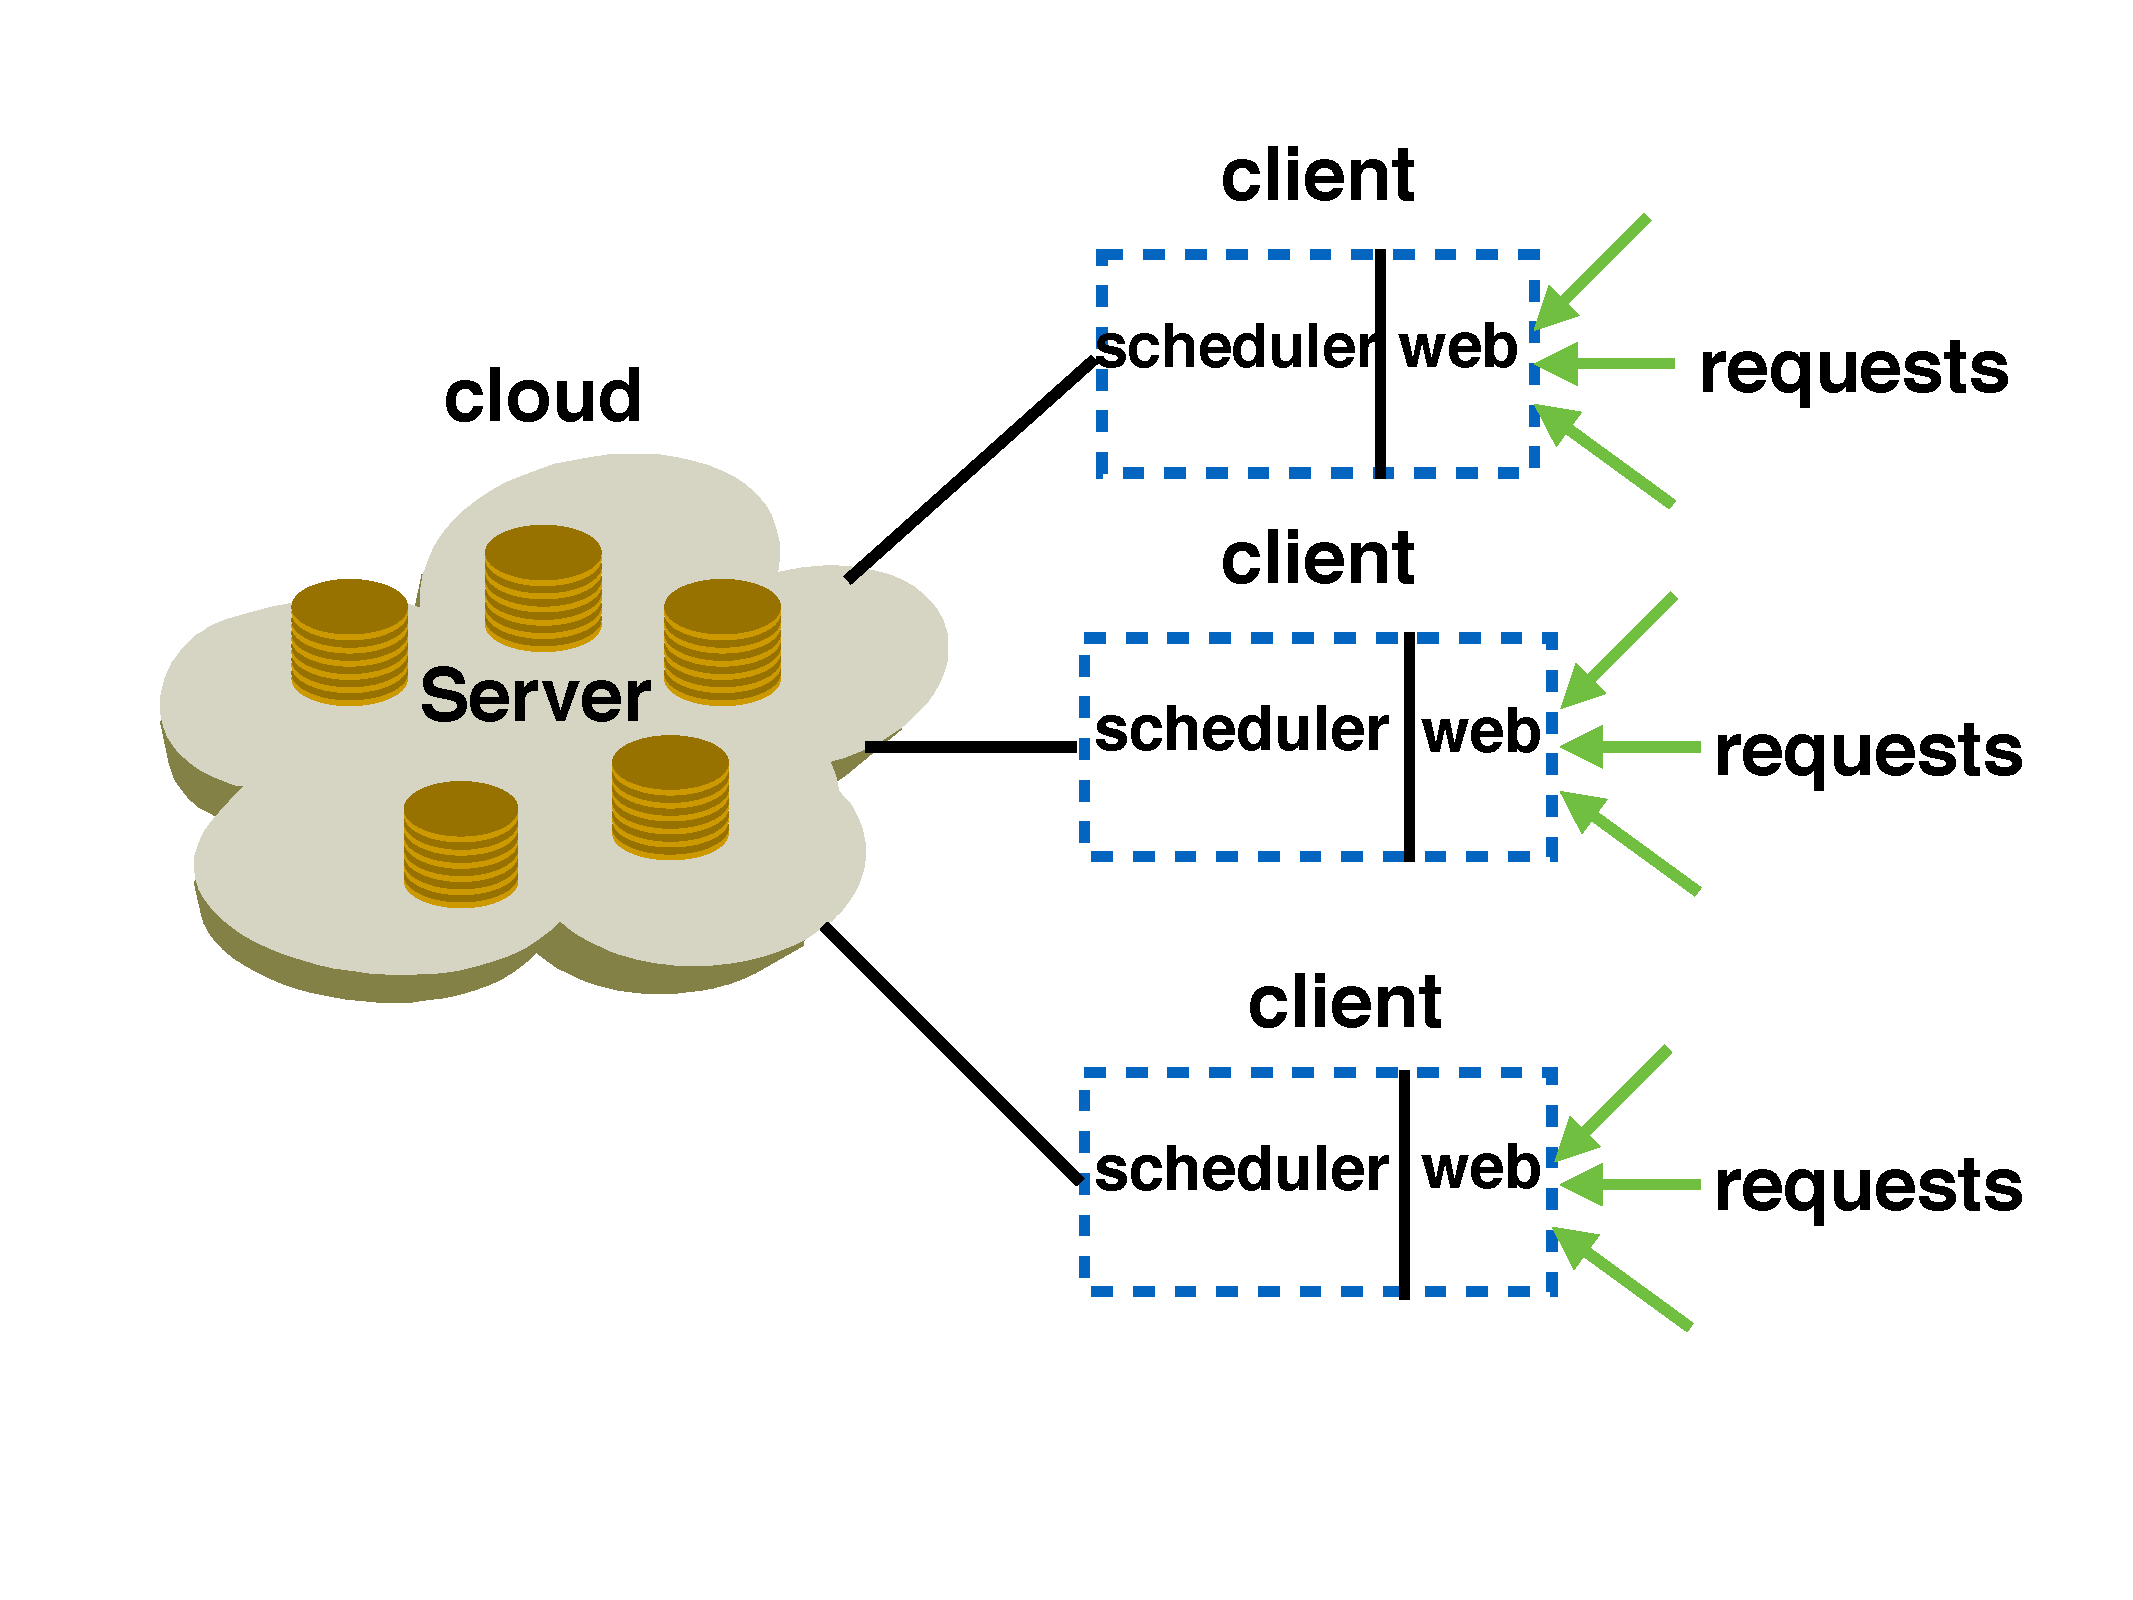
\includegraphics [width=0.8\columnwidth] {figures/DTARGET/picture/motivation/distribute.pdf}
\caption{纠错存储系统的结构图。数据块被存储在云中的机器中,客户端接收用户的请求,然后选择相应的节点来进行数据的组装}
\label{erasure-distribute-fig}
\end{center}
\end{figure}

两个过程影响分布式纠删码存储系统的文件访问速度。
首先,效率低下源选择会导致数据块的选择冲突。
分布式纠删码存储系统总是使用随机源选择请求,
随机源选择可以均分请求,
但是,随机源选择会使一些节点的负载很重,因为节点接入到网络中的带宽是有限的,
使用随机选取数据源的方法会导致很多请求选取同一台机器作为数据块传输的源端,
从而同一台机器上传输负载过重,进而影响任务的传输效率。
为防止这种情况发生,应该选择负载较小的服务器来减少冲突。
其次,TCP不是分布式存储系统的好选择。
TCP是公平的传输方式,但是在纠删码存储系统中,只有客户端接收到所有的数据块才能开始重建文件。
对于TCP传输,不同的块可能获得不同的带宽,最后完成传输的数据块可能会传输的很慢,
这对带宽造成浪费,提前完成的数据传输需要等待后面的传输完成。
如果把早传输完成的数据块的带宽分配给其余的请求任务,那么就能提高链路资源整体利用率。

本章介绍的方法,试图最小化分布式纠删码存储系统的文件平均访问时间(FAT)。
将源选择和数据块传输联合起来进行优化。
首先,提出理想情况下的文件访问时间最小化(Idealized File Access Time Minimization,简称IFATM)问题。
然后忽略源选择,假设数据源是固定的,提出简单理想化的文件访问时间最小化(Simple Idealized File Access Time Minimization,简称SIFATM)问题。
然后,证明即使简单的理想化的问题SIFATM也是NP-hard。
在此之后,提出启发式的“最小负载优先”策略,作为源选择的策略。
对于数据块的传输,提出任务级离线传输方法来决定数据块的传输次序,
并使用最小化期望分配带宽(Minimum-Allocation-for-Desired-Duration,简称MADD)来计算要分配的带宽。
然后设计了一个调度器D-Target,使用它来计算数据块发送需要的带宽。
最后用AT\&T的数据集来测试D-Target的性能。
结果表明,D-Target分别比TCP,Aalo\cite{chowdhury2015efficient},Barrat\cite{dogar2014decentralized}和pFabric\cite{pFabric}性能分别提高了2.5$\times$,1.7$\times$,1.8$\times$,3.6$\times$。
在本章节中做出的贡献是:

(1)提出数据中在分布式纠删码存储系统中,首先,提出将源选择和数据块的传输结合起来进行优化。

(2)提出理想情况下的文件访问时间最小化(Idealized File Access Time Minimization,简称IFATM)问题,
随后,简化IFATM,得到简单理想情况下的文件访问时间最小化(Simple Idealized File Access Time Minimization,简称SIFATM)问题,研究其复杂度,并导出2-近似离线算法,并证明其近似度。随后,本章根据2-近似算法调度思想提出在线调度策略。

(3)设计D-Target,一个调度器来选择有效的信号源并为中继线分配带宽。
实验结果显示,D-Target分别比TCP,Barrat\cite{dogar2014decentralized},
Aalo\cite{chowdhury2015efficient},pFabric\cite{pFabric}提高了2.5$\times$,1.7$\times$,1.8$\times$,3.6$\times$。


\section{研究动机}
\label{erasure_coding:motivation}
\begin{figure}[b]
\begin{center}
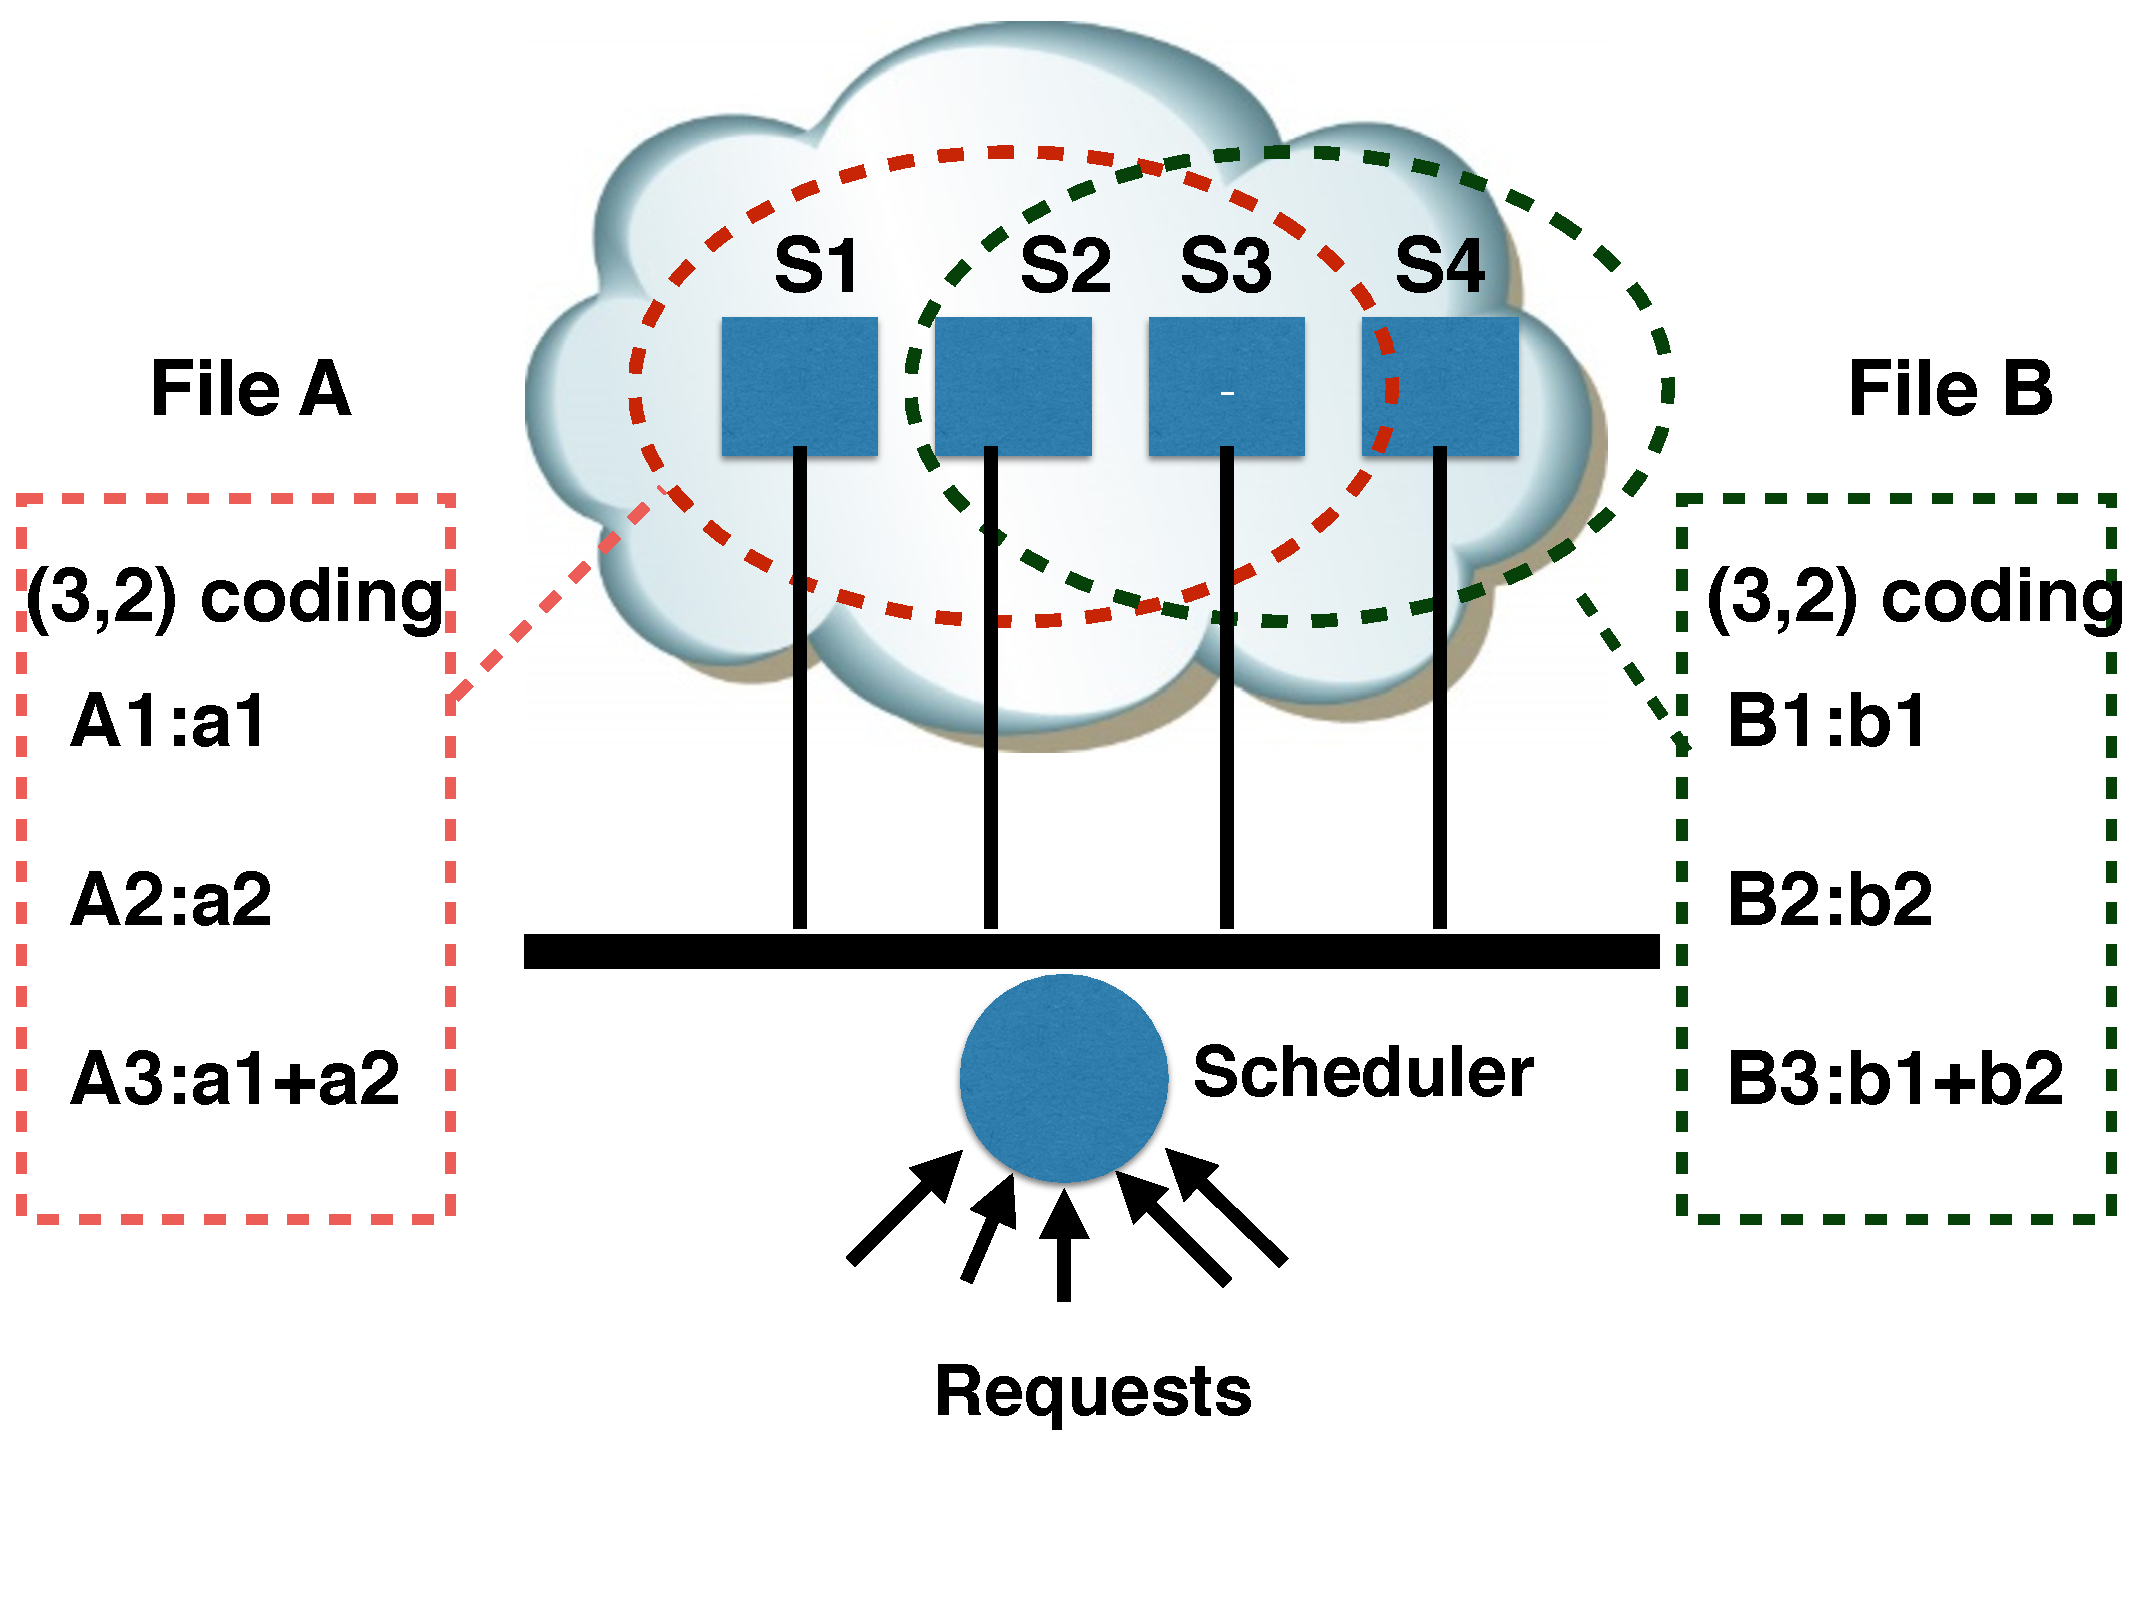
\includegraphics [width=0.8\columnwidth] {figures/DTARGET/picture/motivation/motivation.pdf}
\caption{一个纠删码存储系统,存储了两个文件,使用(3, 2) MDS进行编码}
\label{erasure-motivation-fig}
\end{center}
\end{figure}

根据调查发现,2011年仅用于照片存储的空间已经超过20 PB,
而且每周增加60 TB\cite{beaver2010finding,li2013erasure}。
磁盘上进行着大量的海量存储,每天都可能出现大量故障。
为了弥补数据丢失,保证存储在云中的数据的完整性,
需要对数据进行多分备份,并且将复本存储在多个磁盘。
这样做的优势是可以容忍数据的丢失,因为只要有一个备份可用就能迅速的得到需要的数据\cite{li2013erasure}。
但是,仅仅存储数据的备份,会影响磁盘空间的使用效率。
使用纠删编码将数据编码成块,把数据块分布式存储在集群中,
当用户请求数据时,可以选择其中集群的子集数据块,
通过解码算法,得到相应的数据。
这种方法可以弥补数据丢失,从而保证存储在云中的数据的完整性。

尽管纠删编码存储系统可以保证数据的完整性,但是由于读写数据,系统需要对数据进行编码或解码,
由于CPU的限制,经常导致数据访问延迟高,因为网络访问吞吐量低,\cite{dimakis606049decentralized,lin2012secure,dimakis2010network}主要关注高效编码和解码技术。
通过高效的编码技术,CPU的开销将大大降低。
然而,尽管纠删编码将数据存储为多个编码块,但是当访问文件时,系统必须从数据块的存储集合中选择一定数目的子块来进行文件的重组。
文件数据块的传输过程会给网络增加很大的负担。
事实上,延迟优化已经引起越来越多的关注,甚至谷歌和亚马逊已经公布,每增加500毫秒可能导致$1.2\%$的用户损失\cite{schurman2009user}。
优化传输延迟非常重要,因为这可以改善用户体验,从而增加收入。
现在还有很多方法可以减少应用程序在数据中心的传输延迟。
根据优化的粒度,可以将其划分为流粒度优化和任务粒度优化两种。

DCTCP\cite{DCTCP},D$^2$TCP\cite{D2TCP},L$^2$DCT\cite{L2DCT},PDQ\cite{PDQ},pFabric\cite{pFabric},LPD\cite{LPD},D$^3$\cite{D3}
是流级别的优化方法。DCTCP是公平的共享方法,它试图保持交换机的队列短,以减少队列延迟。
然而,在数据中心,应用对带宽有不同的需求,公平分享不是一个好的选择\cite{LPD}。 
D$^2$TCP,LPD,D$^3$是根据截止期限和网络拥塞情况进行带宽分配方法。
他们设定了明确的截止期限,以适应不同的紧急情况,从而使期限紧的数据流获得的带宽
比期限宽的数据流更多。
结果是,更多的应用程序获得了自己满意的带宽。 
L$^2$DCT,PDQ,pFabric尽量减少平均流量完成时间,认为短流量始终是需要尽快完成传输的。
他们扼制大流的带宽,并将更多的带宽分配给短流。
从而,流的平均完成时间大量减少。
尽管流级别的优化方法在延迟优化方面比TCP强,但是在数据中心网络中,分布式应用总是有并行流,只有流级优化是不够的。 
Barrat\cite{dogar2014decentralized},Varys\cite{chowdhury2014efficient},Aalo\cite{chowdhury2015efficient},sunflow\cite{huang2016sunflow}等任务级别的调度方法将应用程序的流程视为一个整体。 
Barrat\cite{dogar2014decentralized}以FIFO的顺序安排任务,通过动态地改变网络中流的多路复用的级别来避免头部阻塞。 
Varys\cite{chowdhury2014efficient}将应用程序的并行流作为coflow,它使用SEBF调度coflows和MADD执行速率控制,结果平均任务完成时间将减少。 
Aalo\cite{chowdhury2015efficient},sunflow\cite{huang2016sunflow}和CODA\cite{zhang2016coda}事先不需要知道coflow的物理信息(coflow 长度,宽度等)。
在纠删码存储系统中,文件访问会产生并行流,实际中流级别优化是不够的,应考虑任务级别的调度方法来提高传输效率。

纠删编码已经在分布式存储系统中被广泛的使用。
在纠错码存储系统中,文件被编码成数据块,数据块被存储在不同的机器上。
在访问文件时,应该从存储块节点的机器集合中选择机器来重建文件。
从用户角度看,用户关心的是请求获得相应的时间。
请求响应的时间越短,用户获得的体验越好,从而系统获得的用户满意度越高。
但是,云中节点之间,节点接入网络的带宽有限,这会增加用获取文件的时间长度,影响用户的体验。
在本节中,展示了纠删编码存储系统的源选择和任务级传输优化的必要性。


在纠删码存储系统中,文件使用(MDS)码编成块。
文件使用(n,k)MDS编码进行编码时,一个文件被编码并存储在n个存储节点中。
n个节点中任何k个节点都能通过编码运算重新组装成文件。
如图\ref{erasure-motivation-fig}所示,考虑两个文件A和B,它们都被编码并存储在$n = 3$个机器上。
在从\{$S_1$,$S_2$,$S_3$\}中选择的2个不同的节点成功处理之后,可以完成检索文件A的请求。
文件B类似,可以从\{$S_2$,$S_3$,$S_4$\}中选择。
为了简化问题,假设所有链接的容量为1,文件A和文件B的块大小也为1。
首先,考虑在t=0时同时到达的两个请求$R_A$和$R_B$分别取文件A和文件B 。
对于$R_A$,文件A具有3个源选择选项:($S_1$,$S_2$),($S_1$,$S_3$),($S_2$,$S_3$),
而文件B有($S_2$,$S_3$),($S_2$,$S_4$),($S_3$,$S_4$)三个源可供选择。
如果调度器使用随机源选择,则有一种常见的情况是$R_A$选择($S_2$,$S_3$),$R_B$选择($S_3$,$S_4$)。
如果传输策略是TCP,那么$R_A$的文件访问时间为$t_A$ = 2,对于$R_B$,则为$t_A$= 2,那么平均文件访问时间(Average File Access Time,简称AFAT)=2。
但是,如果$R_A$选择($S_1$,$S_2$)和$R_B$选择($S_3$,$S_4$),AFAT=1。
从简单的例子可以看出,对于纠删码存储系统,高效的源选择可以减少AFAT,从而用户体验会更好。

而且,对于分布式存储系统,公平传输的方法TCP并不能达到好的效果。
试想一下简单的情况,文件A有两个请求,$R_{A_1}$到达时间为t = 0,$R_{A_2}$到达时间为t = 0.1。 
$R_{A_1}$选择($S_1$,$S_2$)作为源,$R_{A_2}$选择($S_2$,$S_3$)作为源。
对于TCP传输,$R_{A_1}$的文件访问时间FAT=1.9,$R_{A_2}$的文件访问时间FAT=1.9,所以AFAT=(1.9 + 2.0)/ 2 = 1.95。
但是,如果让$R_{A_1}$具有比$R_{A_2}$更高的优先级。
那么$R_{A_1}$的文件访问时间FAT= 1和$R_{A_2}$的文件访问时间FAT = 2,则AFAT=(1 + 2)/ 2 = 1.5。
因而,在分布式存储系统中,结合任务级优化可以大大减少AFAT。

所以,高效的源选择可以避免单个节点负载过重的情形,
任务级别的传输能够合理利用网络资源,
本章节将这两个问题结合起来进行优化,从而使的AFAT大幅减小。



\section{问题分析和任务级传输优化模型}
\label{erasure_coding:networkmodel}
本节对数据中心任务传输模型进行介绍,首先,本节从数据中心非阻塞模型,以及传输任务等对数据中心任务级传输的模型进行介绍。
随后本节介绍数据中心任务调度问题的复杂度,最后,引入任务的离线调度算法,并证明离线调度算法的近似度。

\subsection{网络模型和传输任务定义}
\begin{figure}[b]
\begin{center}
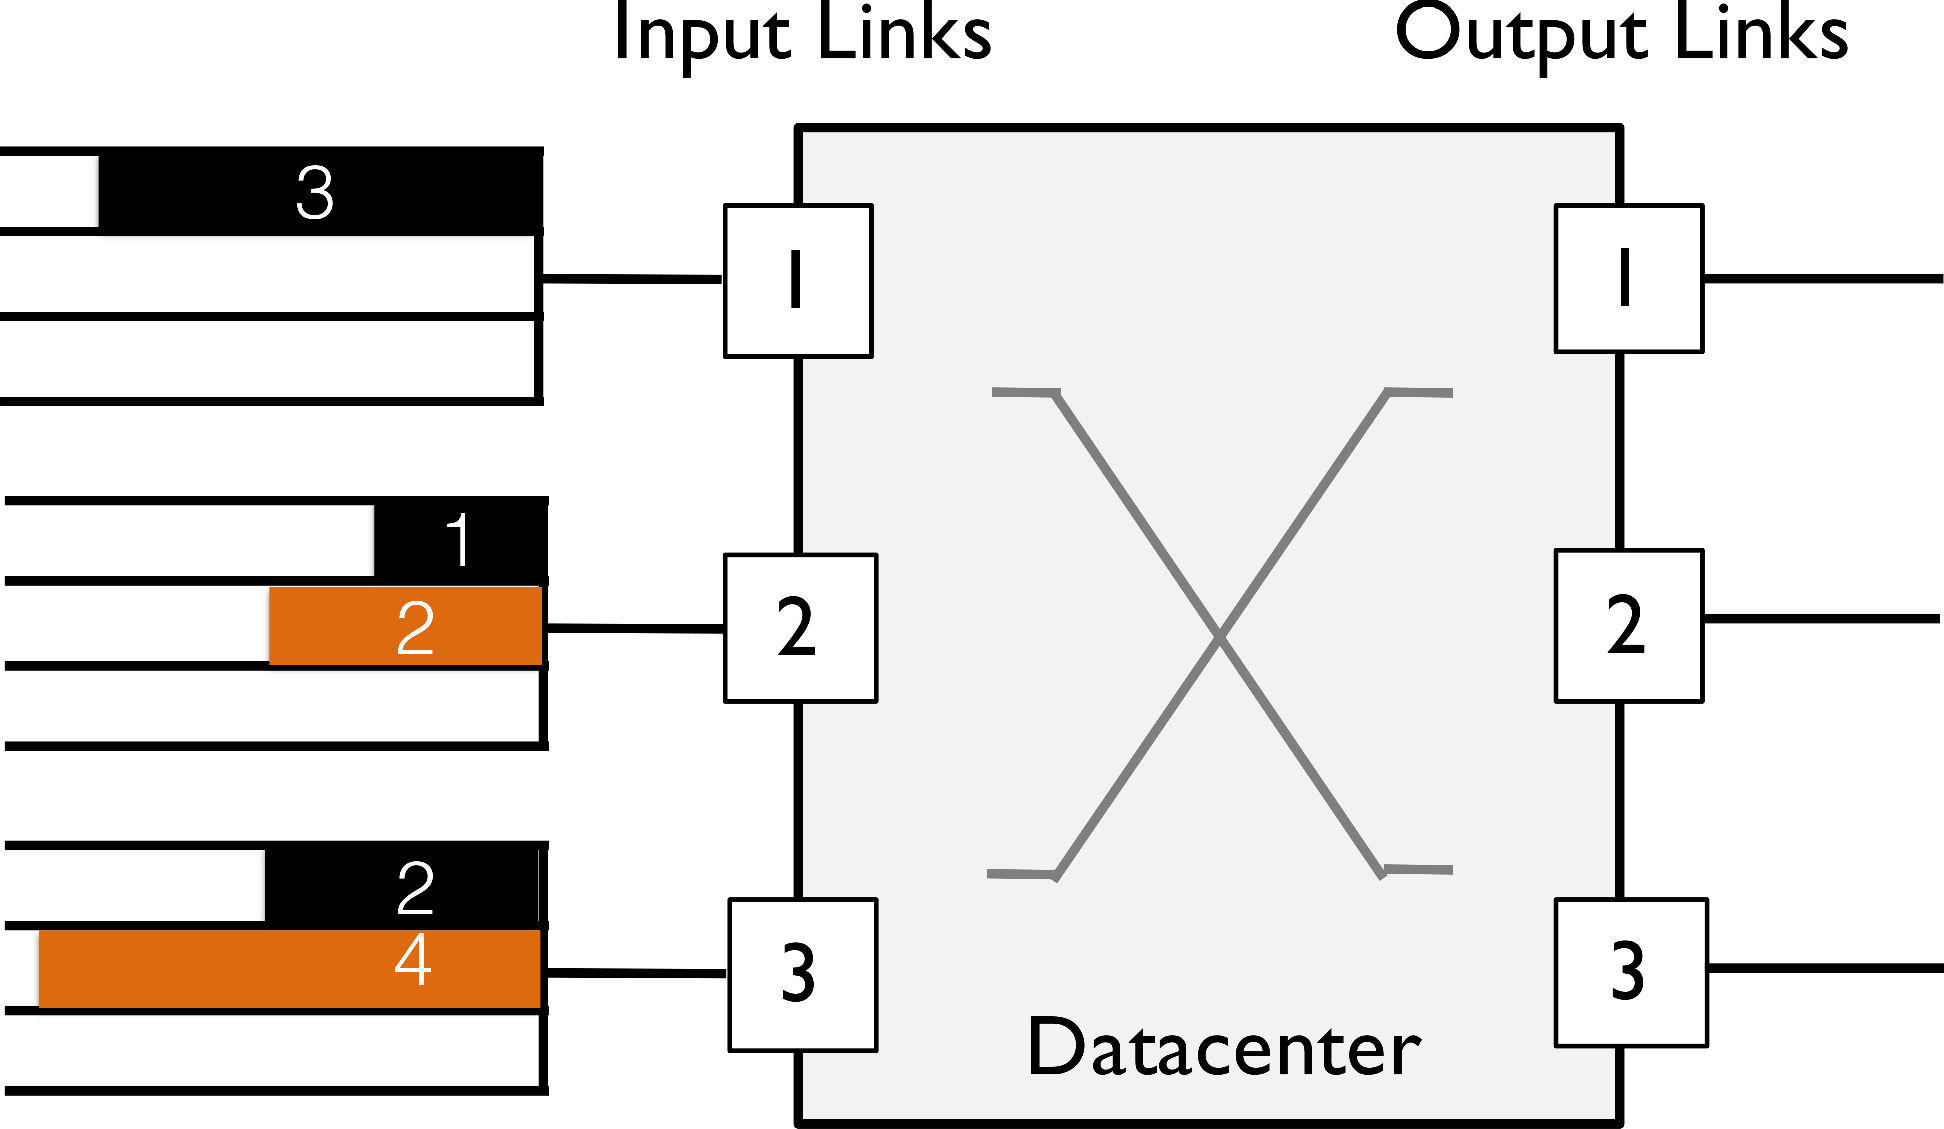
\includegraphics [width=0.8\columnwidth] {figures/others/motivation_color_5.pdf}
\caption{非阻塞的数据中心体系结构}
\label{erasure-non-blocking-fig}
\end{center}
\end{figure}
最近的一些研究方法 \cite{pFabric,chowdhury2014efficient,huang2016sunflow,chowdhury2015efficient},
把数据中心当做一个大型交换机。
如图\ref{erasure-non-blocking-fig}所示,在非阻塞的网络模型中,所有的端口有统一的转发能力,
此外,在此网络模型中,所有的任务竞争交换机的入端口和出端口的带宽。
在本体系结构下,数据中心的内部没有任务的竞争,
只需要在入端口和出端口对任务进行优先级调度即可。
在后面的讨论中,为了简化问题,基于非阻塞体系结构讨论数据中心任务的调度。

定义数据中心的传输任务,
数据中心的传输任务被定义为流组(coflow)\cite{chowdhury2014efficient},
流组是数据流的集合,这些流有共同的目标或者共同需要满足一定的期限等\cite{chowdhury2012coflow,chowdhury2014efficient}。
考虑在$t=0$时,数据中心同时开始传输 $n$条流组,
在非阻塞的网络体系结构下,假设数据中心有$m$台主机,
对应在非阻塞的网络体系结构下有$m$个入端口和$m$个出端口。

下面给出数据中心流组的定义:
 \begin{definition}\label{defination-coflow}
第k个流组$F^{(k)}$,数学上定义为:$F^{(k)}=\{f^k_{i,j}|1 \leq i\leq m,1\leq j \leq m\}$,
$f^k_{i,j}$是每条流的长度(标准化后),机器$i$到机器 $j$。
其中$k$是coflow的序号。
\end{definition}


为了进一步简化问题,假设此“大型交换机”的入端口和出端口的带宽都是1(标准化后)。
所以,当只有这一条流组进行传输时,传输时间是$f^k_{i,j}$ 。
在数据中心中,并不是每一条流组都有$m\times m$条并行的数据流,
如果从机器$i$到$j$没有数据传输,那么$f^k_{i,j}=0$。
下面定义流组的长度和宽度,

 \begin{definition}\label{defination-length}
流组 k的长度\textbf{length($F^{(k)}$)}=$\max \limits_{1 \leq i\leq m,1\leq j \leq m}\{ f^k_{i,j}\}$,即流组中传输时间最长的数据流
\end{definition}



 \begin{definition}\label{defination-width}
定义$b^k_{i,j}$为第k条流组的是否有从机器i到机器j数据传输的标记,
如果$f^k_{i,j}\ne 0$,那么$b^k_{i,j}=1$,否则$b^k_{i,j}=0$。
流组的宽度为:\textbf{width($F^{(k)}$)}=$\sum_{i=1}^m\sum_{j=1}^mb^k_{i,j}$,
即流组 k,$F^{(k)}$的宽度为coflow中最大并行的流的数量。
\end{definition}


\subsection{流组调度和开放并行商店问题}
本部分中,首先讨论开放并行商店问题(Concurrent Open Shop Problem,简称COSP),
然后讨论数据中心传输任务调度的问题复杂度。
\subsubsection{开放并行商店问题}\label{concurrent-open-shop}
开放并行商店模型的定义如下。
考虑一组机器M=\{1,2,...m\},每个机器可以处理一种类型的操作。
定义任务集合N=\{1,2,..n\},每个任务有m个子任务需要完成,
每个机器处理一个子任务。
机器之间相互独立。
当所有机器上的子任务完成时,此任务完成。
设$C_j$表示第j个任务的完成时间。
设置$w_j$为第j个任务的权重,
问题的优化目标为$\mathop {\min }\sum_{j=1}^n w_j\times C_j$

使用 $w_k$表示coflow的权重,权重在实际当中可以表示为coflow $F^{(k)}$的重要性,$C_k$为coflow k的完成时间,
定义如下的理想化权重流组完成时间优化问题(Idealized Weighted Coflow Completion Time Minimization,简称IWCCTM) 问题:

\begin{eqnarray}
& {\rm minimize} & \sum_{k=1}^{n} w_{k} C_{k} \label{eq:WCCO-SC} \\
& {\rm s.t.} &\forall k,j:  \sum_{\forall l:C_l \leq C_k}\sum_{i=1}^{m}f_{i,j}^{(l)} \leq C_k  \label{eq:ingress_constraint}\\
&&\forall k,i: \sum_{\forall l:C_l \leq C_k}\sum_{j=1}^{m}f_{i,j}^{(l)} \leq C_k   \label{eq:egress_constraint}
\end{eqnarray}

IWCCTM目标是最小化权重流组完成时间之和,
其中(\ref{eq:ingress_constraint})和(\ref{eq:egress_constraint})是对入端口和出端口有带宽的限制。
对于一个流组 $F^{(k)}$,完成时间是$C_k$,考虑在$F^{(k)}$完成之前的流组的集合:$F^{(l)}$:$C_l \le C_k$。
对于任意的入端口 $i$ (或者出端口$j$),在这个端口上的所有流的传输时间,
至少为:$\sum_{j=1}^{m}f_{i,j}$ (出端口 $j$上的为:$\sum_{i=1}^{m}f_{i,j}$),这个值应该小于$C_k$。
下面证明在只允许非抢先调度的情形下,任务的权重完成时间之和的问题是NP-hard的。

下面本文证明,在只允许非抢先调度的情形下,任务的权重完成时间之和的问题是NP-hard的。

 \begin{lemma}\label{IWCCTM-proof2}
 如果只允许非抢先调度,那么IWCCTM问题和开放商店中任务的权重完成时间之和的问题是等价的,问题的复杂度是NP-hard。
\end{lemma}

\begin{proof}
开放商店可以被描述为:有一系列的机器 $M = \{1,...,m\}$,
每台机器能执行一种类型的操作,
任务集合表示为$N = \{1,...,n\}$,每个任务需要特定的$m$类的操作。
每个任务 $j \in N$有一个权重$w_j \in R > 0$,并且任务$j$在机器$i$ 上的处理时间是$p_{ij} \in R\ge0$。
当一个任务在机器上的所有操作都完成了,才能认为这个任务完成。
特别的,一个任务的所有的操作能够并行的处理。

对于一个$m \times m$的数据中心,根据定义(\ref{defination-coflow})可以得到一条流组 $F^{(k)}$,
聚合每个端口发出的数据流,得到数据中心传输子任务的定义:

\begin{equation}
\label{coflow-subtask}
 L_l^{(k)}=\left\{
\begin{array}{rcl}
\sum_{i=1}^{m}f_{i,l}^{(k)}& {0      \le l   <m} \\
\sum_{j=1}^{m}f_{l-m,j}^{(k)} & {m      \le l   <2m} \\
\end{array} \right. 
\end{equation}

因为数据中心有$2m$个端口,因此每个流组有$2m$个传输子任务。
考虑开放商店中有$n$ 个任务和$2m$台转发能力相同的机器,每个任务有$2m$个子任务,每个子任务需要在一台机器上执行。
每个流组可以和每个任务对应,每台机器的子任务执行和每个传输子任务对应。
因为已经被证明,在开放商店中最小化任务权重完成时间是NP-hard\cite{mastrolilli2010minimizing}\cite{chen2000supply}\cite{roemer2006note}\cite{Qiu2016Experimental},
因此,在非阻塞网络中对流组的调度问题的复杂度也是NP-hard。
\end{proof}


\subsection{离线算法和近似度证明}
对于在开放商店中解决任务权重完成时间,
当前最优的解决方法是2-近似的贪心策略\cite{mastrolilli2010minimizing,kumar2011lp}。
因为IWCCTM问题和开放商店任务权重完成时间有很近的关系,
引入一个如算法\ref{IWCCM-offline}所示的离线非抢先调度算法。




\begin{algorithm}
\KwIn{流组集合 $\mathcal{F}=\{F^{(k)}\}$,权重集合$\mathcal{W}=\{\overline{w_k}=w_k\}$, $1 \le k \le n$; } 
\KwOut{a permutation $\gamma$ of $\{1, \dots, n\}$;}
$\mathcal{P} \gets \{1, \dots, 2m\}$, $\mathcal{R} \gets \{1, \dots, n\}$\;
 $L_i^{(k)}= \sum_{j=1}^mf_{i,j}^{(k)}$  for $1 \le k \le n$ and $i \le m$\;
  $L_{j+m}^{(k)}= \sum_{i=1}^mf_{i,j}^{(k)}$ for $1 \le k \le n$ and $ j \le m$\;
 $L_p=\sum_{1 \le k \le n}L_p^{(k)}$ for each $p \in \mathcal{P}$\;
   \For{$i$ from $n$ to $1$ }{
   $p^*=\arg \max \limits_{p \in \mathcal{P}}L_p$\;
    $\gamma[i]=r^*=\arg\min \limits_{r \in \mathcal{R}} \overline{w_r}/L_{p^*}^{(r)}$\;
     $\theta=w_{r^*}/L_{p^*}^{(r^*)}$\;
     $\mathcal{R} = \mathcal{R} \setminus \{r^*\}$\;
    $\overline{w_r} = \overline{w_r}-\theta \times L_{p^*}^{(r)}$ for all $r \in \mathcal{R}$\;
    $L_p=L_p-L_p^{(r^*)}$ for all $p \in \mathcal{P}$\;
  }
  \textbf{return} $\gamma$;
  \caption{解决IWCCM的2近似算法}
  \label{IWCCM-offline}
 \end{algorithm}
 
 
 算法\ref{IWCCM-offline}首先构造了端口集合 $\mathcal{P}=\{1, \dots, 2m\}$,
 这个集合对应着非阻塞网络体系结构的“巨型交换机”的$m$个入端口和$m$个出端口,
 行1$\sim$4,计算了每个端口的负载。
 然后算法迭代的找出第i个循环下要调度的流组,循环是按照倒叙进行。
 在每轮迭代中,首先找出负载最重的端口$p^*$,然后找到这个端口上有最小的权重和负载比的流组(coflow),
 保存这个流组的负载到$\gamma[i]$(行 6 $\sim$ 7),
 随后更新要调度的流组的集合,以及要调度的coflow集合的权重,和端口的负载(行8 $\sim$ 11),
 随后,进行下一轮的迭代。
 
 可以很明显的看出,算法\ref{IWCCM-offline}产生序列$\gamma$ 的复杂度是$O(n(m+n))$,
 其中m是数据中心中端数量,n是任务的数量。
 
下面证明算法\ref{IWCCM-offline}的是2-近似,根据Chen\cite{chen2000supply},
 IWCCTM中有如下限制:
 \begin{eqnarray}
  &\forall j \leq 2m, S \subset F: \sum_{k=1}^{|S|} L_{j}^{(k)} C_{k} \geq \frac{1}{2}\sum_{k=1}^{|S|} (L_{j}^{(k)})^2+ \frac{1}{2}(\sum_{k=1}^{|S|} L_{j}^{(k)})^2
\end{eqnarray}
其中F是要调度的coflow的集合,$L_{j}^{(k)}$是coflow k 在端口j的传输时间,
$|S|$是集合S的长度,因此,IWCCTM可以表述为:
 \begin{eqnarray}
 & {\rm minimize} & \sum_{k=1}^{n} w_{k} C_{k} \label{eq:WCCO-SC2} \\
& {\rm s.t.} &\forall j \leq 2m, S \subset F: \sum_{k=1}^{|S|} L_{j}^{(k)} C_{k} \geq \frac{1}{2}\sum_{k=1}^{|S|} (L_{j}^{(k)})^2+ \frac{1}{2}(\sum_{k=1}^{|S|} L_{j}^{(k)})^2  \label{eq:IWCCM-SC3}
\end{eqnarray}

基于此,得到IWCCTM的对偶函数为:
 \begin{eqnarray}\label{IWCCTM4}
 & {\rm maximize} & \sum_{j=1}^{2m}\sum_{S\subset F}\left [\frac{1}{2}\sum_{k=1}^{|S|} (L_{j}^{(k)})^2+ \frac{1}{2}(\sum_{k=1}^{|S|} L_{j}^{(k)})^2 \right ] y_j^S\label{eq:WCCO-SC4} \\
& {\rm s.t.} & \forall k\leq n:\sum_{j=1}^{2m} L_{j}^{(k)} \sum_{S\subset F:k=1}^{|S|} y_j^S=w_k  \label{eq:IWCCM-SC5}\\
& & \forall  y_j^S\geq 0  \label{eq:IWCCM-SC6}
\end{eqnarray}

为了证明算法\ref{IWCCM-offline}的是2-近似,引入以下引理:
 \begin{lemma}\label{IWCCTM-proof3}
 对任意的j$\leq $2m和S$\subset$F,有($\sum_{k=1}^{|S|}L_{j}^{(k)})^2\leq (2-\frac{2}{n+1})\left [ \frac{1}{2}\sum_{k=1}^{|S|} (L_{j}^{(k)})^2+ \frac{1}{2}(\sum_{k=1}^{|S|} L_{j}^{(k)})^2 \right ]$
\end{lemma}

基于此,有如下定理:

 \begin{theorem}\label{IWCCTM5}
 算法\ref{IWCCM-offline}的近似度是$(2-\frac{2}{n+1})$,其中n是并行的coflow的数目
 \end{theorem}

\begin{proof}
使用$p(i)$表示在第6行中第i个循环中中选出的端口,
使用$\theta(i)$表示在第8行中第i个循环计算的$\theta$值,
使用$\overline{w_r(i)}$表示第10行中第i个循环中调整的权重,
使用$\gamma(i)$表示第i循环起始时没有调度的流组集合。
有$\gamma(i)=\{r^*(1),r^*(2)...r^*(i)\}$,
其中$r^*(i)$表示流组的id,
定义如下的对偶解,对于任意的j$\leq $2m和S$\subset$F

\begin{equation}
\label{duiou}
 y_j^S=\left\{
\begin{array}{rcl}
\theta(i) &\text{j=p(i),S=$\gamma(i)$,i=1,2,3...n}\\
0 &\text{其它情况}\\
\end{array} \right. 
\end{equation}
(\ref{duiou})是(\ref{IWCCTM4})的对偶解,是因为:
\begin{eqnarray}\label{proof_equal}
\sum_{j=1}^{2m} L_{j}^{r^*(i)} \sum_{S\subset F} y_j^S
&\overset{(a)}{=}&\sum_{l=i}^{n}  L_{p(l)}^{r^*(i)} y_{r^*(l)}^S\nonumber \\
&\overset{(b)}{=}&\sum_{l=i}^{n}  L_{p(l)}^{r^*(i)} \theta(l)\nonumber \\
&\overset{(c)}{=}& w_{r^*(i)}-\overline{w_{r^*(i)}}\nonumber \\
&\overset{(d)}{=}&w_{r^*(i)}
\end{eqnarray}
(a) 成立是因为算法1是从n到1开始循环的, 因此第i个循环的计算结果可以通过i+1个循环到n个循环推算得到。
(b) 成立是因为有解(\ref{duiou})成立,
(c)成立是因为在第i个循环,r$\in \gamma(i)$有 
\begin{equation}
w_r^{(i)}=w_r-\sum_{l=k}^{n}L_{p(l)}^r\theta(l)
\end{equation}
(d)成立是因为对于任意的k=1,2..n,有$\overline{w_{r^*(l)}}=0$。
通过(\ref{proof_equal}),可以得知,解(\ref{duiou})满足(\ref{eq:IWCCM-SC5})。
此外,从算法\ref{IWCCM-offline}输入得知,$\overline{w_{r^*(l)}}$初始化值为权重初始值,
算法\ref{IWCCM-offline}第7行和第10行知,每个循环选出最小的权重负载比,
因此,第10行中,$\theta \geq 0$,因此公式(\ref{eq:IWCCM-SC6})成立。
下面证明算法\ref{IWCCM-offline}的近似度是$(2-\frac{2}{n+1})$。
注意,算法\ref{IWCCM-offline}调度的coflow满足:
$C_{\gamma[1]} \leq C_{\gamma[2]} \leq... C_{\gamma[n]}$,
根据步骤6,7,对所有的i=1,2,..n,有$C_{\gamma[i]}=\sum_{j=1}^i L_{p^*(i)}^{r^*(j)}$。
令$(C_k^{CP})_{k \in \mathcal{F}}$是最优解,$(C_k^{*})_{k \in \mathcal{F}}$是最优解向量。
调度的最优化解为:


\begin{align}\label{proof_optimization}
&\sum_{k=1}^{n} w_{k} C_{k}\nonumber \\
=&\sum_{k=1}^{n} (\sum_{j=1}^{2m} L_{j}^{(k)} \sum_{S\subset F} y_j^S )C_{k}\nonumber \\
=&\sum_{j=1}^{2m} \sum_{S\subset F} y_j^S\sum_{k \in S}L_{j}^{(k)}C_k \nonumber \\
=&\sum_{l=1}^{n} y_{p^*(l)}^{\gamma(l)}\sum_{g=1}^{l} L_{p^*(l)}^{g}C_g\nonumber \\
=&\sum_{l=1}^{n} y_{p^*(l)}^{\gamma(l)}\sum_{h=1}^{l} L_{p^*(l)}^{r^*(h)}C_{r^*(h)}\nonumber \\
\overset{(e)}{\leq} &\sum_{l=1}^{n} y_{p^*(l)}^{\gamma(l)}C_{r^*(l)}\sum_{h=1}^{l} L_{p^*(l)}^{r^*(h)}\nonumber \\
\overset{(f)}{=} &\sum_{l=1}^{n} y_{p^*(l)}^{\gamma(l)}(\sum_{h=1}^{l} L_{p^*(l)}^{r^*(h)})^2\nonumber \\
\overset{(g)}{\leq}& (2-\frac{2}{n+1})\sum_{l=1}^{n}y_{p^*(l)}^{\gamma(l)}\{ \frac{1}{2}\sum_{h=1}^{l} \left[L_{p^*(l)}^{r^*(h)}\right]^2+ \frac{1}{2}\left[\sum_{h=1}^{l} L_{p^*(l)}^{r^*(h)}\right]^2 \}\nonumber \\
\overset{(h)}{\leq}& (2-\frac{2}{n+1}) \sum_{k=1}^{n} w_{k} C_{k}^{CP} \nonumber \\
\leq& (2-\frac{2}{n+1}) \sum_{k=1}^{n} w_{k} C_{k}^{*} 
\end{align}

(e)成立因为对于h=1,2,...l,有$C_{r^*(h)}\leq C_{r^*(l)} $,(f)成立,因为$C_{r^*(l)}=\sum_{h=1}^{l} L_{p^*(l)}^{r^*(h)}$,
(g)成立因为有引理\ref{IWCCTM-proof3}成立,(h)成立因为y是(\ref{IWCCTM4})$\sim$(\ref{eq:IWCCM-SC6})的解。
因此算法\ref{IWCCM-offline}的近似度是$(2-\frac{2}{n+1})$,其中n是并行的流组的数目
\end{proof}

\section{纠删码存储系统传输优化算法和分析}
\label{erasure_coding:algorithm}
在本节中,在假设数据中心是非阻塞网络体系结构的基础上讨论纠删码存储系统中传输优化问题。
首先,提出理想化文件访问时间最小化问题(Idealized File Access Time Minimization,简称IFATM)。
然后对纠删码存储系统进行算法设计和分析。
\subsection{问题定义}
考虑一个由n个存储节点组成的非阻塞数据中心,用
$\mathcal{S} = \{s_1,s_2,...s_n\}$ 表示这些节点的组合。
用$\mathcal{F}=\{b_1,b_2,b_3..b_r\}$ 表示存储在机器集合中的r个文件集合。
使用$(n_i,k_i)$-MDS纠删码,将文件$b_i$生成相同大小的$n_i $个不同的数据块,并把不同的数据块存储在$n_i$台机器上。 
当获取文件时,从$n_i$台机器中任意$k_i$台机器都能够获得文件。
$(n_i, k_i)$-MDS纠删码也引入了一个冗余因子 $n_i / k_i$。 
用$\mathcal{C}=\{c_1,c_2...c_m\}$表示m个客户的集合。
假设所有$L$ 个请求在时间0到达,并且用$T^{(k)}_{b^k}$表示第 $k$个请求获取文件$b^k(b^k\in \mathcal{F})$。
第$k$个请求得到的响应$T^{(k)}_{b^k} $是一个流组(coflow), $T^{(k)}_{b^k}=\{f_{i,j}^{(k,b^k)}|1 \le i \le n ,1\le j \le m\}$,
其中 $f_{i,j}^{(k,b^k)}$表示一个大小为$f_{i,j}^{(k,b^k)}$的流。
$x^{(k,b^k)}_{i,j}  \in \{0,1\}$ ,用1表示存在从服务器$i$到客户端$j$的流。
0表示从服务器$i$到客户端$j$没有流。
由于非阻塞模型的入口和出口端口的转发能力是\textbf{单位1},
所以流$f_{i,j}^{(k,b^k)}$的传输时间是$f_{i,j}^{(k,b^k)}$。
理想情况下的非抢先调度文件访问时间最小化问题-Idealized File Access Time Minimization (IFATM)可以定义为:


 \begin{eqnarray}
&\d {\rm minimize} & \sum_{g=1}^{L} C_{g} \label{eq:ECSF-SC} \\
& \d{\rm s.t.} &\forall g,j\sum_{\forall l:C_l \leq C_g}\sum_{i=1}^{n}f_{i,j}^{(l,b^l)}*x_{i,j}^{(l,b^l)}\leq C_g  \label{eq:ingress_constraint2}\\
&&\forall g,i\sum_{\forall l:C_l \leq C_g}\sum_{j=1}^{m}f_{i,j}^{(l,b^l)}*x_{i,j} ^{(l,b^l)} \leq C_g   \label{eq:egress_constraint2}\\
&& \forall l,j\sum_{i=1}^nx_{i,j}^{(l,b^l)}=k_{b^l}  \label{eq:source_constraint}
\end{eqnarray}

目标是最小化文件平均访问时间。
约束条件(\ref{eq:ingress_constraint2}) 和(\ref{eq:egress_constraint2}) 主要是端口转发能力的限制。
优化目标是最小化文件平均访问时间。
对于一个请求,$T^{(k)}_{b^k}$,请求的完成时刻是$C_{k}$ ,考虑到在这个时刻之前完成的文件传输的集合, $T^{(l)}_{b^l}$: $C_{l} \le C_{k}$。
对于任何一个入端口(或者出端口),这个端口上的文件平均访问时间至少是 $\sum_{\forall l:C_l \leq C_g}\sum_{i=1}^{n}f_{i,j}^{(l,b^l)}*x_{i,j}^{(l,b^l)}$(或者$\sum_{\forall l:C_l \leq C_g}\sum_{j=1}^{m}f_{i,j}^{(l,b^l)}*x_{i,j} ^{(l,b^l)}$ ),不应该比$C_{k}$要大。
(\ref{eq:source_constraint})是源选择的限制:对于文件${b^l}$,调度器要从$k_{b^l}$个机器中选择合适的机器集合。

非抢先调度文件访问时间最小化问题(IFATM)问题是NP-hard的。
为了证明此,考虑一个简单的情况,假设在一组请求中,有(1)$n_i = k_i $,此时$x_{i,j} ^{(l,b^l)}=1$(2)$n_i $和服务器总数相同,
即每个服务器都存储文件编码的一个数据块。
进一步假设所有的请求同时到达。
得到简单非抢先调度文件访问时间最小化问题(Simple Idealized File Access Time
Minimization,简称SIFATM):
 \begin{eqnarray}
&\d {\rm minimize} & \sum_{g=1}^{L} C_{g} \label{eq:simple_ECSF-SC} \\
& \d{\rm s.t.} &\forall g,j\sum_{\forall l:C_l \leq C_g}\sum_{i=1}^{n}f_{i,j}^{(l,b^l)}\leq C_g  \label{eq:simple_ingress_constraint}\\
&&\forall g,i\sum_{\forall l:C_l \leq C_g}\sum_{j=1}^{m}f_{i,j}^{(l,b^l)} \leq C_g   \label{eq:simple_egress_constraint}
\end{eqnarray}

 \begin{lemma}\label{theorem-SIFATM}
简单非抢先调度文件访问时间最小化问题(SIFATM)是NP-hard问题。
\end{lemma}
\begin{proof}
把公式(\ref{eq:WCCO-SC})$\sim$(\ref{eq:egress_constraint})中权重设置为1,
那么SIFATM和IWCCTM问题相同,根据引理\ref{IWCCTM-proof2},IWCCTM的复杂度是NP-hard,因此,SIFATM也是NP-hard。
\end{proof}

事实上,将算法\ref{IWCCM-offline}中权重均设置为1,算法\ref{IWCCM-offline}即为SIFATM的一个2-近似算法。
算法\ref{IWCCM-offline}是一个理想的情况,因为它假定所有请求都同时到达,并且文件每个服务器为存储每个文件的一个数据块。
事实上,在现实世界中,请求可以在任何时候到达,并且不是每个机器上都存储了要请求的文件的数据块,
文件只存储机器的一个子集。 
在此情形下,算法\ref{IWCCM-offline}在实际中难以使用。

现实中,对文件的请求会随时到达,并且端口的负载是在随时变化的,此外任务的分配是负载均衡的\cite{dean2008mapreduce,dogar2014decentralized,luo2016towards}。
因此,调度器可以不考虑端口负载的差异性 (\textbf{近似 1})。
此外,对于分布式的纠删码存储系统,每个客户端有每个文件压缩的数据块的数据块大小 (\textbf{事实 1}),因此,只需要在服务器端计算
端口的负载即可。
此外,对于纠删码存储系统,每个数据块的大小相同,因此,可以通过数据压缩比来计算要传输的数据块的大小 (\textbf{事实 2})。
定义文件$b_d$的压缩比为 $\alpha_{b_d}=\frac{chunk\ size \ of \ b_d}{file \ size \ of \ b_d}$,算法\ref{online-algorithm}是一个在线调度策略。

\begin{algorithm}
\KwIn{活跃的请求集合$\mathcal{T}$, 为文件已经选好的集合 $\theta_{b^k}^{(k)}=\{x_{1,1} ^{(k,b^k)},x_{1,2} ^{(k,b^k)}...x_{i,j}^{(k,b^k)}...\} ,\forall T^{(k)}_{b^k} \in \mathcal{T},\forall x_{i,j}^{(k,b^k)} \in \{0,1\},i \le n,j \le m$,  文件压缩比 $\alpha=$ \{$\alpha_{b_1},\alpha_{b_2}..\alpha_{b_r}$\}, 文件大小集合$\beta=\{\beta_{b_1},\beta_{b_2},..\beta_{b_r}\}$, 新到达的请求 $T_{b^c}$}
\KwOut{$\gamma$}
 $\theta_{b^c}= SourceSelection(\mathcal{T},\theta,\alpha,\beta,T_{b^c})$\;
 $\mathcal{T} = \mathcal{T} \cup \{T_{b^c}\}$\;
$L_i^{(d)}= \sum_{j=1}^{m}\alpha[b^d]*\beta[b^d]*x_{i,j}^{(d,b^d)}$ for $\forall d \in \mathcal{T},i \le n$\;
$L_{j+n}^{(d)}= \sum_{i=1}^n\alpha[b^d]*\beta[b^d]*x_{i,j}^{(b,b^d)}$ for $\forall d \in \mathcal{T},j \le m$\;
$l^{(d)}$=$ \max \limits_{1 \le i \le n+m}L_i^{(d)}$ for $\forall d \in\mathcal{T}$ \;
$\pi^{(d)}$=1/$l^{(d)}$ for $\forall d \in \mathcal{T}$ \;
对[$\pi^{(1)}$,$\pi^{(2)}$,$\pi^{(3)}$...]非降序排列,然后把排序后的结果给 $\gamma$\;
  \textbf{return} $\gamma$;
\caption{在线调度算法}
\label{online-algorithm}
\end{algorithm}

当一个新的文件请求到达时,算法\ref{online-algorithm}被调用。
算法\ref{online-algorithm}的输入是 $\mathcal{T},\theta_{b^k}^{(k)},\alpha,\beta,T_{b^c}$,其中$\mathcal{T}$ 是活跃的文件请求集合。
$\theta_{b^k}^{(k)}$包含源节点集合和$T^{(k)}_{b^k}$的目标客户端。
$\alpha$ 是存储每个系统中文件大小的集合,$\beta$ 是每个文件的压缩比,$T_{b^c}$是新到达的请求。
算法\ref{online-algorithm}的第1行是为这个新到达的请求选择合适的选源节点,
第3$\sim$5行为每个在集合$\mathcal{T}$中的请求计算负载。
第3行计算的是服务器端的负载,第4行计算的是客户端的负载。
特别的,使用$\alpha[b^d]*\beta[b^d]*x_{i,j}^{(d,b^d)}$来计算文件$b^d$的块大小。
第5行计算每个请求的负载,请求的完成时间是由最后一条流的完成时间决定的。
第6行计算请求$T^{(c)}_{b^c}$的完成时间,同样的请求的完成时间是由最后一条流的完成时间决定的。
第7行是对请求$\pi^{(1)}$,$\pi^{(2)}$,$\pi^{(3)}$...进行非降序排序,然后把排序的结果反馈给$\gamma$。
第8行,算法将计算的结果返回。
%\begin{figure}[b]
%\begin{center}
%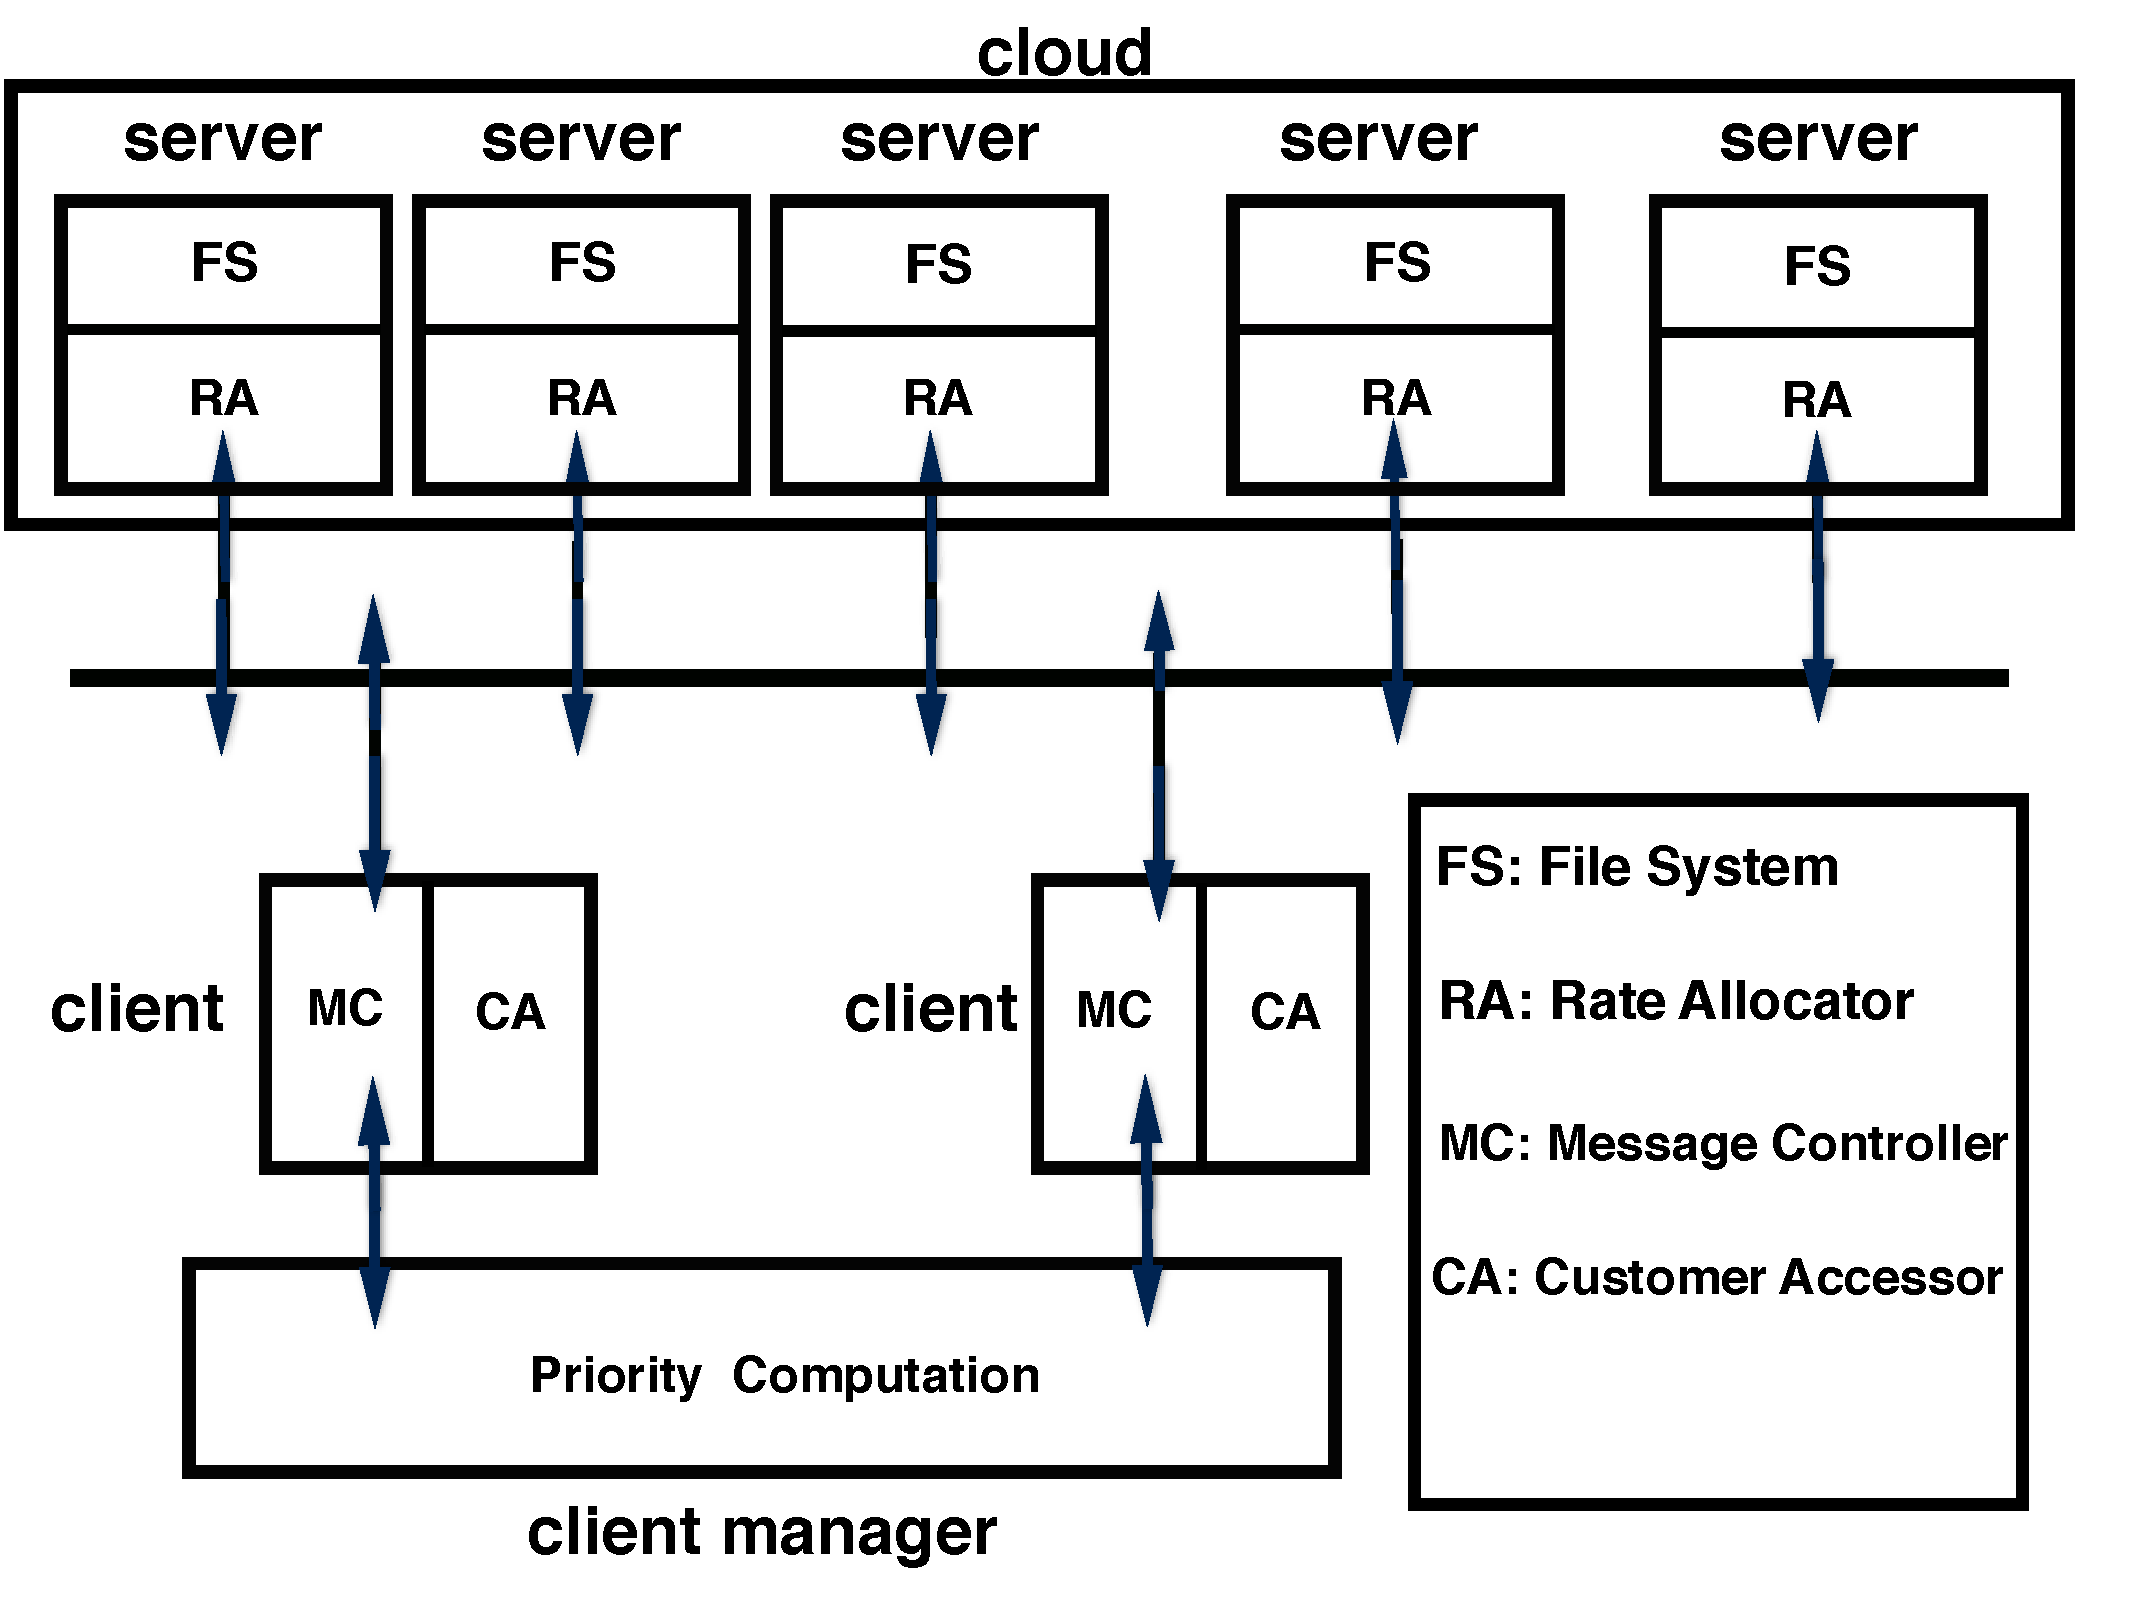
\includegraphics [width=0.8\columnwidth] {figures/DTARGET/picture/system/System.pdf}
%\caption{D-Target系统设计}
%\label{erasure-system-fig}
%\end{center}
%\end{figure}

\subsection{源选择问题}
\begin{algorithm}
\KwIn{活跃的请求集合$\mathcal{T}$, 为文件已经选好的集合 $\theta_{b^k}^{(k)}=\{x_{1,1} ^{(k,b^k)},x_{1,2} ^{(k,b^k)}...x_{i,j}^{(k,b^k)}...\} ,\forall T^{(k)}_{b^k} \in \mathcal{T},\forall x_{i,j}^{(k,b^k)} \in \{0,1\},i \le n,j \le m$,  文件压缩比 $\alpha=$ \{$\alpha_{f_1},\alpha_{f_2}..\alpha_{f_r}$\}, 文件大小集合t $\beta=\{\beta_{f_1},\beta_{f_2},..\beta_{f_r}\}$, 新到达的请求 $T_{b^c}$}
$B_i= \sum_{\forall b \in \mathcal{T}}\sum_{j=1}^{m}\alpha[b^d]*\beta[b^d]*x_{i,j}^{(d,b^d)}$, for $i \le n$ 并且机器b存储 $T_{b^c}$的数据块\;
对B采用非降序排列\;  
选择前$k_{b^c}$个数据块,并且把相应的$x_{i,j}^{(c,b^c)}$设置为1, 其他的设置成0,然后把所有的$x_{i,j}^{(c,b^c)}$添加到 $\theta_{b^c}$\;
\textbf{return} $\theta_{f^c}$;
\caption{最小负载优先策略}
\label{source-selection-algorithm}
\end{algorithm}

算法\ref{source-selection-algorithm}中,第1行计算入端口的负载。
然后第2行对负载进行非将排序,第3行选择负载最小的$k_{b^c}$源并且把$x_{i,j}^{(c,b^c)}$设置成1。
对其他的端口的这个值设置为0。
最后,把所有的$x_{i,j}^{(c,b^c)}$加到$\theta_{b^c}$ 集合中,然后返回$\theta_{b^c}$。

算法\ref{source-selection-algorithm}尝试从所有的源节点中选择负载最小的源节点。
认为这是有意义的,因为,文件的获取时间FAT是由传输最慢的数据块决定,
因为FAT是由传输最慢的数据块决定的,因此,最小负载优先的策略可以减少文件平均获取时间。 


\subsection{D-Target的设计}
\begin{algorithm}
\KwIn{ 活跃的请求集合$\mathcal{T}$, 为文件已经选好的集合 $\theta_{b^k}^{(k)}=\{x_{1,1} ^{(k,b^k)},x_{1,2} ^{(k,b^k)}...x_{i,j}^{(k,b^k)}...\} ,\forall T^{(k)}_{b^k} \in \mathcal{T},\forall x_{i,j}^{(k,b^k)} \in \{0,1\},i \le n,j \le m$,  文件压缩比 $\alpha=$ \{$\alpha_{b_1},\alpha_{b_2}..\alpha_{b_r}$\}, 文件大小集合 $\beta=\{\beta_{b_1},\beta_{b_2},..\beta_{b_r}\}$, 新到达的请求 $T_{b^c}$}
\KwOut{所有活动数据块的带宽}
根据算法 \ref{online-algorithm},对 $\mathcal{T}$和新来的请求$T^{(k)}_{b^k}$进行排序\;
根据算法 \ref{bandwidth-compuataion-algorithm}给$\mathcal{T}$分配带宽\;
对所有端口的任务$\mathcal{T}$分配剩余的带宽\;
发送$r_{i,j}$给对应的服务器\;
\caption{客户端管理器的操作过程}
\label{scheduler}
\end{algorithm}
为了实现对纠删码存储系统的调度,本文设计D-Target。
D-Target有三个主要部件,客户端管理器,客户端信息收集器,服务器速率分配器。
D-Target采取集中式的调度器,调度器尝试最小化文件平均访问时间(AFAT)。
因为,服务器端的负载可以通过客户端的信息进行计算,所以调度器只需要对客户端进行管理。
\subsubsection{客户端管理器}
在D-Target中,客户端管理器是系统的核心,
当有请求到达时,它计算请求的优先级 (Algorithm \ref{online-algorithm}) 然后选择合适的源 (算法 \ref{source-selection-algorithm})。
计算完每个文件请求的优先级,D-Target计算每个数据块的带宽,客户端管理器方法如算法\ref{scheduler}所示。
在算法\ref{scheduler}中,当一个新的文件请求到达时,客户管理器对所有活动的请求根据算法 \ref{online-algorithm} (行1)进行排序(行2)。
最后,如果链路还存在剩余带宽,那么把剩余带宽分给数据块,然后把相应的结果发给对应的服务器(第3行$\sim$第4行)。

\begin{algorithm}
\KwIn{ 已经排好序的集合$\gamma$, 端口集合的剩余带宽集合 $Rem(.)$}
\KwOut{每个数据块的剩余带宽, 端口带宽剩余能力集合$Rem(.)$}
\For{k $\in \gamma$ }{
根据(\ref{weight_completion_gamma})计算负载$g^{(k)}$\;
 \For{$f_{i,j}^{(k,b^k)}$$ \in k$ }{
$r_{i,j}=f_{i,j}^{(k,b^k)}/g^{(k)}$\;
$Rem(P_i^{(in)})-=r_{i,j}$\;
 $Rem(P_j^{(out)})-=r_{i,j}$\;
 }
}
\textbf{return} 每个数据块的带宽,端口剩余带宽集合 $Rem(.)$ 
\caption{带宽计算的过程}
\label{bandwidth-compuataion-algorithm}
\end{algorithm}



\begin{eqnarray} \label{weight_completion_gamma}
g^{(k)}=\max(\max \limits_i \frac{ \sum_{j=1}^mf_{i,j}^{(k,b^k)}}{Rem(P_i^{(in)})},\max \limits_j \frac{ \sum_{i=1}^nf_{i,j}^{(k,b^k)}}{Rem(P_j^{(out)})})
\end{eqnarray}

算法 \ref{bandwidth-compuataion-algorithm}展示了带宽计算的细节。
对每个已经排好序的请求, (\ref{weight_completion_gamma})计算出瓶颈链路的完成时间(第2行)。
对于其他文件的数据块,使用瓶颈链路数据块的完成时间当做这个文件传输的数据块(第4行)。
最后,更新每个端口的剩余带宽(第6行$\sim$第7行)。

\subsubsection{客户端}
客户端存储文件的信息,包括数据块的位置,大小等。
客户端和用户进行交互,并且收集文件请求的信息,最后,把这些信息发送给客户端管理器。
服务器端存储所有的数据块,他们接受来自客户端获取文件的请求,
然后根据客户端计算的结果来控制每条数据流发送的带宽。


\section{实验验证}
\label{erasure_coding:evaluation}
在本节中,通过真实使用真实的数据中心的流量来彻底评估D-Target的性能。
本节的主要结果可以概述为:

(1)使用AT\&T的数据中心的流量,发现D-Target性能比TCP,Aalo\cite{chowdhury2015efficient},Barrat\cite{dogar2014decentralized}和pFabric\cite{pFabric}分别提高2.5$\times$,1.7$\times$,1.8$\times$,3.6$\times$。

(2)不使用最小负载优先(Smallest-Load-First,简称SLF)启发式源选择,D-Target性能分别比TCP,Barrat,Aalo,pFabric高1.9$\times$,1.4$\times$,1.6$\times$,2$\times$。以最小负载优先(Smallest-Load-First,简称SLF)启发式源选择,TCP,Barrat \cite{dogar2014decentralized},Aalo\cite{chowdhury2015efficient},pFabric \cite{pFabric}比没有SLF的方法效果好$30\%$,$27\%$,$33\%$,$20\%$。

(3)离线场景下,与2-近似的离线算法相比,在线算法的性能损失少于$15\%$。






\subsection{仿真测试}
本部分在大多数实验中使用AT\&T中心的流量。
这些数据流量是从AT\&T的数据中心的60个机架的720个服务器收集来的,包括文件大小,数据块的大小,每个文件的块位置以及30天的请求。

\textbf{评价指标}。使用平均文件访问时间(Average File Access Time, 简称AFAT)来评估不同调度方法的有效性。
考虑文件的特定类别的平均FAT。 
FAT涵盖了从调度程序的时间选择源到客户端接收所有的块。
将D-Target与四个典型的比较
调度算法:TCP,Aalo\cite{chowdhury2015efficient},Barrat\cite{dogar2014decentralized}和pFabric\cite{pFabric},使用TCP作为基准,相对于TCP的性能提高定义为 = $\frac{baseline \, \,  of \,  avg \,  FAT}{current \,   avg \,  FAT}$

\textbf{开源}。为了使本部分实验可复原,发布了D-Target的主要代码。 
D-Target的代码可以在\cite{DTARGET}下载。

\subsection{真实流量仿真}
\begin{figure}[h]
\centering
\subcaptionbox{平均FAT对比}
 {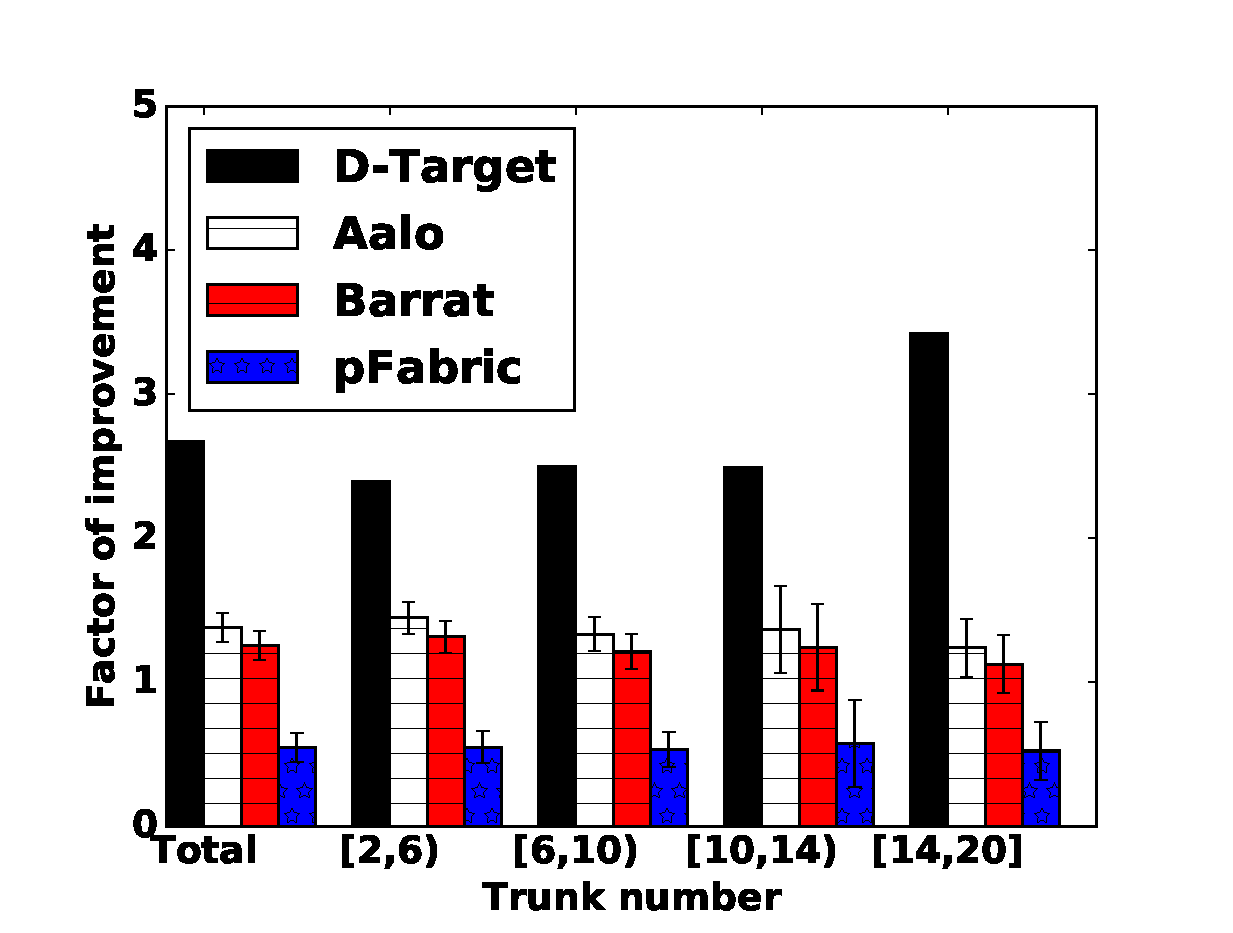
\includegraphics[width=0.32\columnwidth]{figures/DTARGET/picture/evaluation/ex1/total.eps}}
\subcaptionbox{平均FAT(使用SLF策略选源)}
{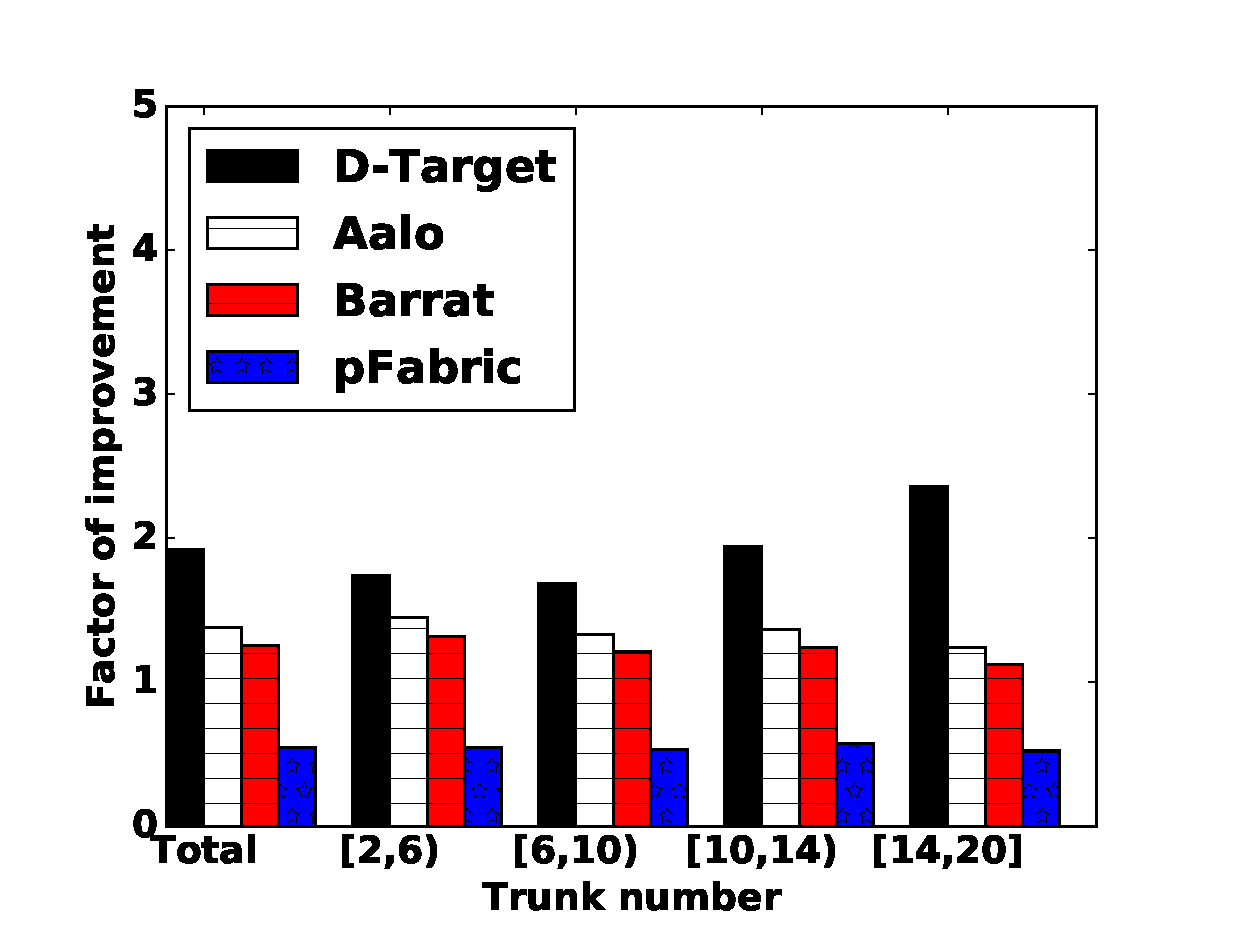
\includegraphics[width=0.32\columnwidth]{figures/DTARGET/picture/evaluation/ex1/random_select.eps}}
\subcaptionbox{使用SLF和不使用SLF结果对比}
{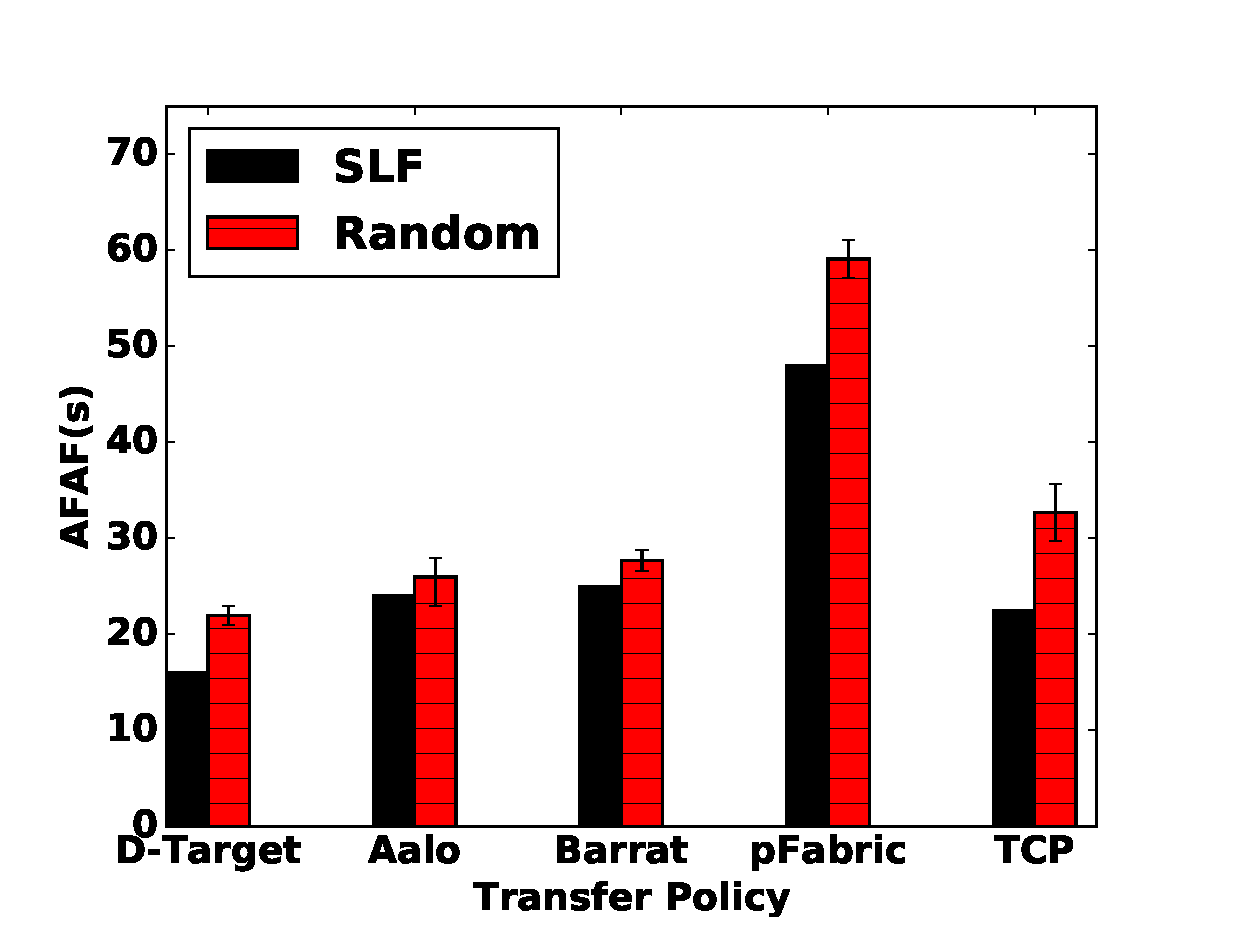
\includegraphics[width=0.32\columnwidth]{figures/DTARGET/picture/evaluation/ex1/diff.eps}}
\caption{使用AT\&T流量的实验结果,使用TCP当做基准。注意,对于一些随机选取的结果,每次实验的结果会不同,为了弥补这些不同,每组实验运行100次,取每次的平均值}
\label{trace_fig}
\end{figure}


在这一部分,用AT\&T的纠删码系统的数据来测试D-Target的性能。
对于源选择,因为每次源可能不相同,而SLF选取的源相同。
为了消除随机的源选择出现的波动,每组实验运行100次,图\ref{trace_fig}显示了实验结果。
注意,在每组的实验结果中,error bar表示的是平均值,最大值,最小值。


图\ref{trace_fig}(a)显示了AFAT的结果。
可以看到,D-Target相对TCP提高2.5$\times$,而对于Aalo,Barrat,pFabric相对TCP提高分别是1.5$\times$,1.2$\times$,0.8$\times$。
对于分布式纠删码存储系统,响应包含并行数据块,根据响应的宽度将其分为四组。
当并行块数分别为[2,6],[6,10],[10,14]和[14,20]时,
可以看到D-Target相对于TCP的改进倍数分别为2.2$\times$,2.4$\times$,2.8$\times$,3$\times$。
Aalo相对于TCP的改进倍数分别为1.5$\times$,1.4$\times$,1.42$\times$,1.5$\times$。
Barrat相对于TCP的改进倍数分别为1.3$\times$,1.5$\times$,1.2$\times$,1.15$\times$。
pFabric相对于TCP的改进倍数分别为0.6$\times$,0.53$\times$,0.6$\times$,0.7$\times$。
随着块并行度的增加,改善的幅度变得更大。
这是因为,并行块数越多,请求之间的冲突越高,
所以进行源选择和流量控制的必要性越大。

在现代的纠删码存储系统中,当请求到达时,调度器总是使用随机源选择来选择那些源。
在本文中,以最小负载优先算法来选择源。
在此情形下,会发生较少的碰撞。
图\ref{trace_fig}(b)显示了所有传输方法使用最小负载优先的启发式来选择数据源的结果。
可以看到D-Target和其他方法对比,优势变小。
平均而言D-Target,Aalo,Barrat比TCP分别提高1.9$\times$,1.5$\times$,1.3$\times$。
当并行块数分别为[2,6],[6,10],[10,14]和[14,20]时,
可以看到D-Target相对于TCP的改进倍数分别为1.8$\times$,1.7$\times$,1.9$\times$,2.2$\times$。
Aalo相对于TCP的改进倍数分别为1.2$\times$,1.3$\times$,1.4$\times$,1.5$\times$。
Barrat相对于TCP的改进倍数分别为1.1$\times$,1.4$\times$,1.3$\times$,1.4$\times$。

图\ref{trace_fig}(c)显示了不同方法的平均文件访问时间(FAT)比较。
可以看到,D-Target,Aalo,Barrat,pFabric,TCP使用最小负载优先策略进行源选择分别比
随机源选择性能提高大约$30\%$,$30\%$,$27\%$,$33\%$,$20\%$。



\subsection{不同设置下性能}
在这一部分,探讨D-Target在不同参数下的性能。
知道FAT是受源选择和数据块传输影响的。
对于分布式纠删编码存储系统,采用(n,k)MDS编码进行编码,
其中n表示文件编码的块数,k表示重建文件所需的块数,k和n决定文件传输的宽度。
因为要探索每个参数对系统性能的的影响,所以在每组实验中,
除了要探究的参数之外,其余参数设置为默认值。
表\ref{default-parameter}显示了每个实验的默认设置。
在默认参数中有512个文件,文件大小在100KB到10GB之间。 
MDS的默认参数值是(8,4),每个请求的到达时间在0到1000s之间。
实验中的入口和出口端口容量是1GB。
对于每组实验,生成参数100次,绘制出最大值,最小值,平均值。

\begin{figure}[h]
\centering
\subcaptionbox{平均FAT对比}
 {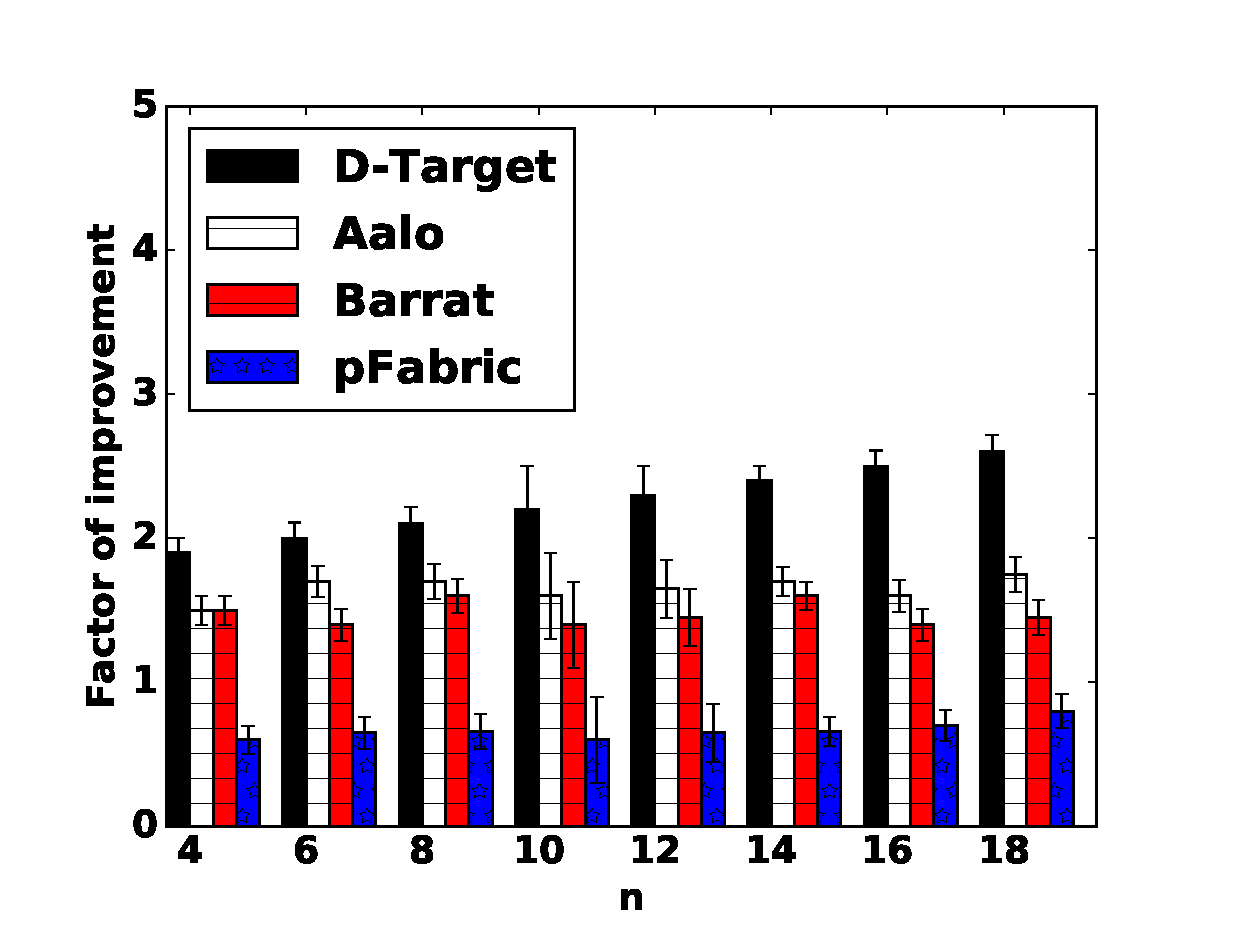
\includegraphics[width=0.32\columnwidth]{figures/DTARGET/picture/evaluation/ex2/M.eps}}
\subcaptionbox{平均FAT对比}
{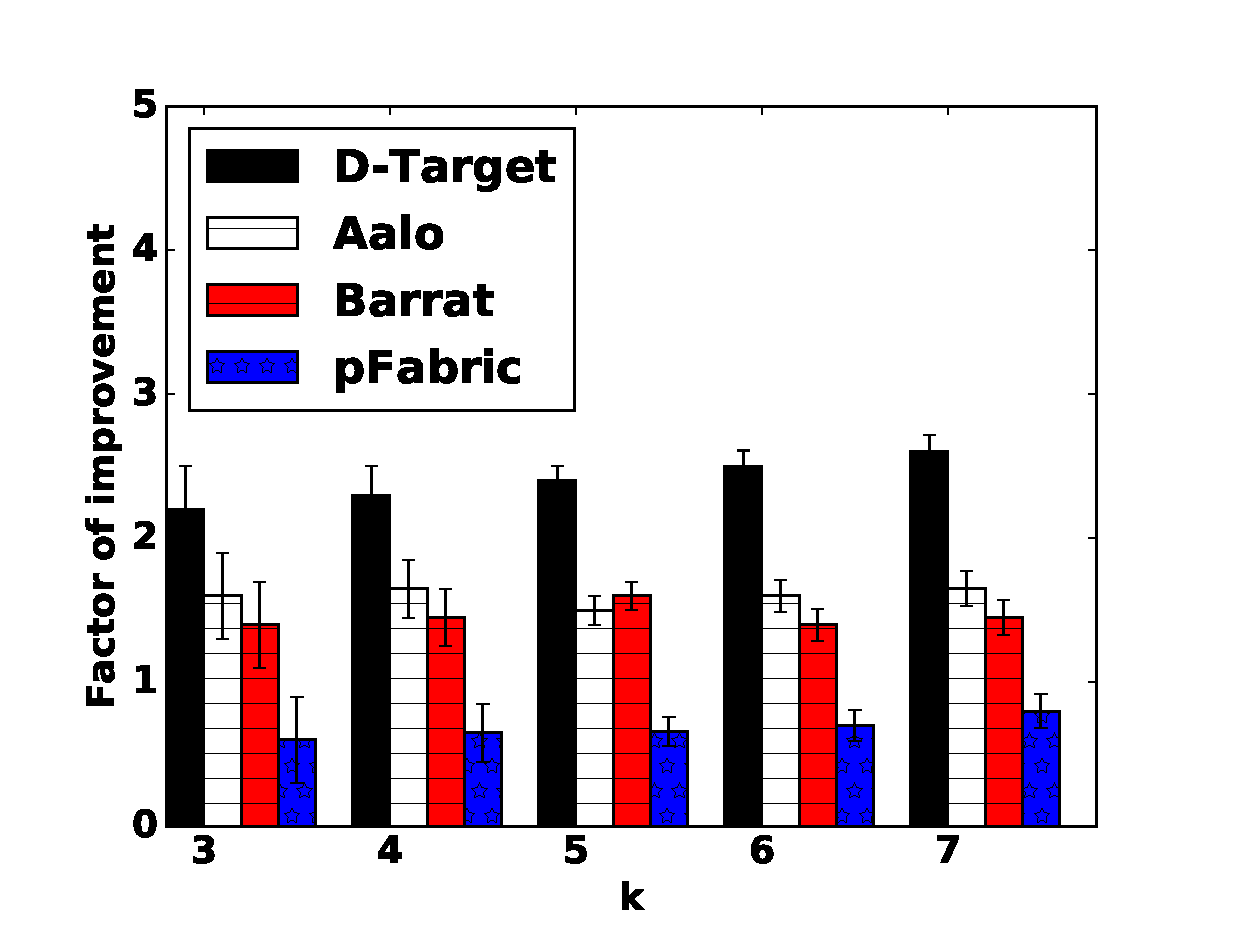
\includegraphics[width=0.32\columnwidth]{figures/DTARGET/picture//evaluation/ex2/N.eps}}
\subcaptionbox{平均FAT对比}
{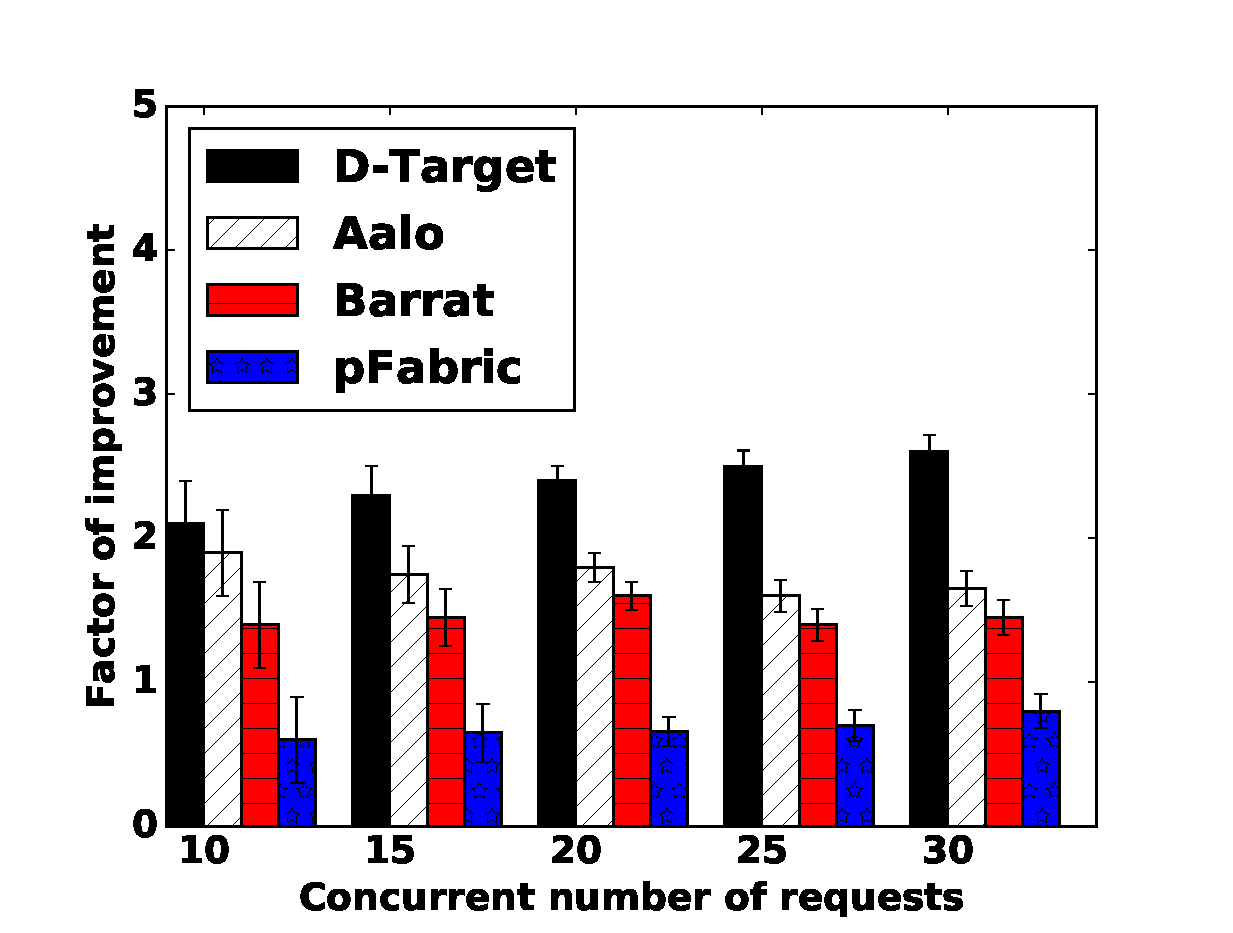
\includegraphics[width=0.32\columnwidth]{figures/DTARGET/picture//evaluation/ex2/alpha.eps}}
\caption{平均FAT对比,注意TCP被当做基准}
\label{settings_fig}
\end{figure}

 
 \begin{table}[h]
\centering
\caption{各组实验的缺省参数}\label{default-parameter}
\renewcommand{\arraystretch}{1.5}
\begin{tabular}{|c|c|c|c|c|c|c|c|} \hline
\setlength{\tabcolsep}{10pt}
  请求的数量 &  文件的大小 & n & k &$\alpha$ &链路容量 &请求到达时间 \\ \hline
 512&  [100KB,10GB] & 8 & 4 &1.5&1GB&[0s,1000s]\\ \hline
\end{tabular}
\end{table}

图\ref{settings_fig}(a)显示随着n的增加,D-Target相对于TCP提高的幅度变大。
当n=4时,D-Target相对于TCP提高1.8$\times$,Aalo是1.5$\times$,Barrat相对于TCP提高1.5$\times$,
当n=6时,D-Target相对于TCP提高的幅度是1.9$\times$,Aalo相对于TCP提高的幅度是1.6$\times$,Barrat相对于TCP提高的幅度是1.4$\times$,
当n=8时,D-Target相对于TCP提高的幅度是2.0$\times$,Aalo相对于TCP提高的幅度是1.7$\times$,Barrat相对于TCP提高的幅度是1.5$\times$。
而当n=18时,D-Target相对于TCP提高的幅度是2.5$\times$,Aalo是1.5$\times$,Barrat相对于TCP提高的幅度是1.3$\times$。
可以看到,D-Target在更大的n值时表现更好,这是n越大,节点之间的冲突变得更高,所以需要更好地优化源选择和更高效的传输。
 
图\ref{settings_fig}(b)显示随着k的增加,D-Target性能更好。
当k=3时,D-Target相对于TCP提高的幅度2.1$\times$,Aalo相对于TCP提高的幅度是1.5$\times$,Barrat相对于TCP提高的幅度是1.6$\times$,
当k=4时,D-Target相对于TCP提高的幅度是2.2$\times$,Aalo相对于TCP提高的幅度是1.6$\times$,Barrat相对于TCP提高的幅度是1.7$\times$,
当k=7时,D-Target相对于TCP提高的幅度是2.5$\times$,Aalo相对于TCP提高的幅度是1.52$\times$,Barrat相对于TCP提高的幅度是1.72$\times$。
k越大时,D-Target性能更好,因为,k越大,D-Target由于较少的冲突而性能提高。

实际上,实际系统中请求可以随时到达。
请求到达时间可能会影响数据中心网络中的网络负载。
图\ref{settings_fig}(c)显示出了输并发对系统性能的影响。
当并行传输的数据块数目为10时,D-Target相对于TCP提高的幅度2.1$\times$,Aalo相对于TCP提高的幅度是1.9$\times$,Barrat相对于TCP提高的幅度是1.5$\times$,
当并行传输的数据块数目为15时,D-Target相对于TCP提高的幅度是2.2$\times$,Aalo相对于TCP提高的幅度是1.8$\times$,Barrat相对于TCP提高的幅度是1.6$\times$,
而当并行传输的数据块数目为30时,D-Target相对于TCP提高的幅度是2.5$\times$,Aalo相对于TCP提高的幅度是1.54$\times$,Barrat相对于TCP提高的幅度是1.52$\times$。
可以看到,对于较大的并发请求数量,D-Target的性能提高不断增加。
这是因为网络负载越重,根据优先级调度的必要性增加。

\subsection{离线算法和在线算法之间的差异}
\begin{figure}[h]
\setlength{\abovecaptionskip}{0pt} 
\setlength{\belowcaptionskip}{1pt} 
  \centering%
  \subcaptionbox{平均FAT对比\label{DTARGET_Evaluation_Motivation:subfig1}} %标题的长度,超过则会换行,如下一个小图。
    {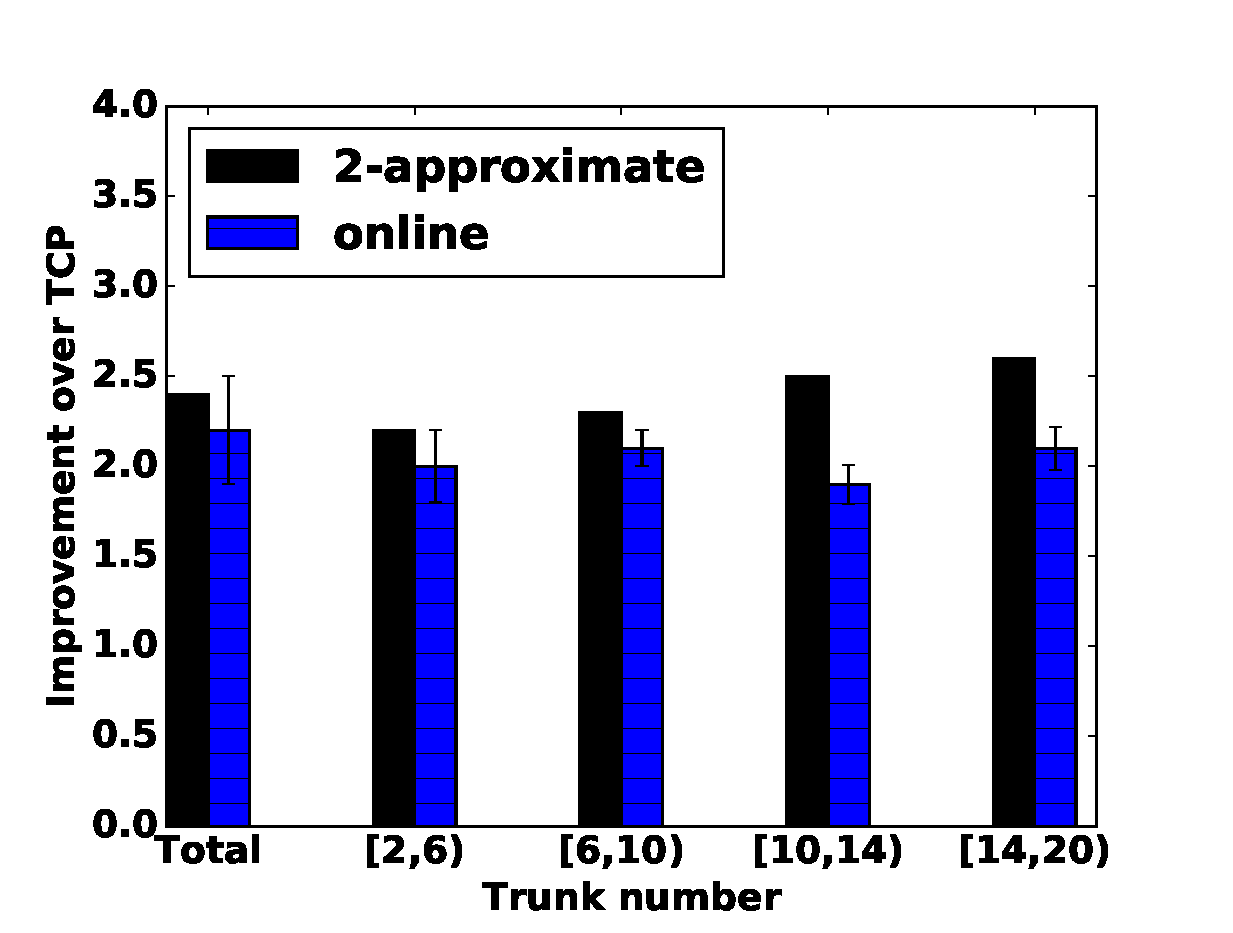
\includegraphics[width=0.5\columnwidth]{figures/DTARGET/picture/evaluation/ex3/on_off_2.eps}}%
  \subcaptionbox{FAT分布\label{DTARGET_Evaluation_Motivation:subfig2}}
      {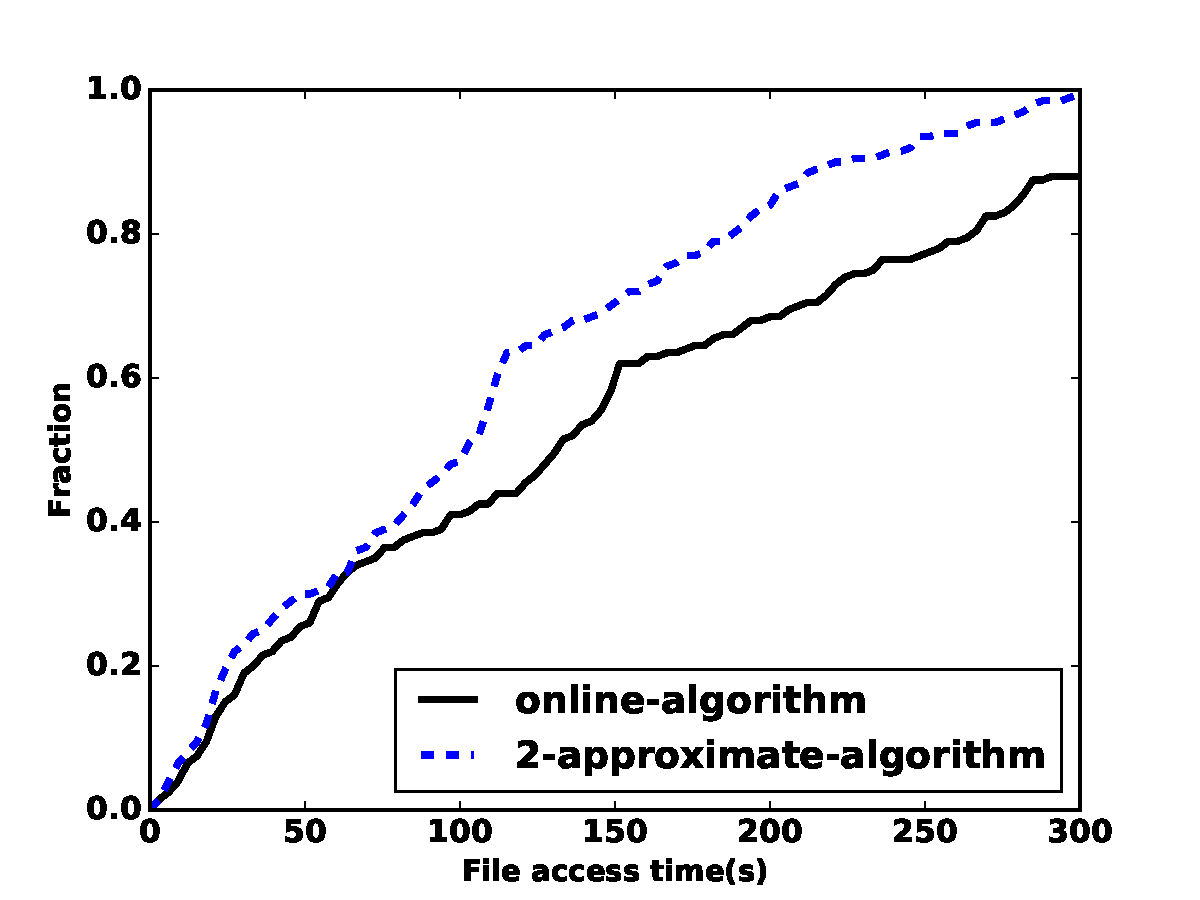
\includegraphics[width=0.5\columnwidth]{figures/DTARGET/picture/evaluation/ex3/online_offline.pdf}}
  \subcaptionbox{平均FAT(没有使用SLF)\label{DTARGET_Evaluation_Motivation:subfig3}}%标题的长度,超过则会换行,如下一个小图。
    {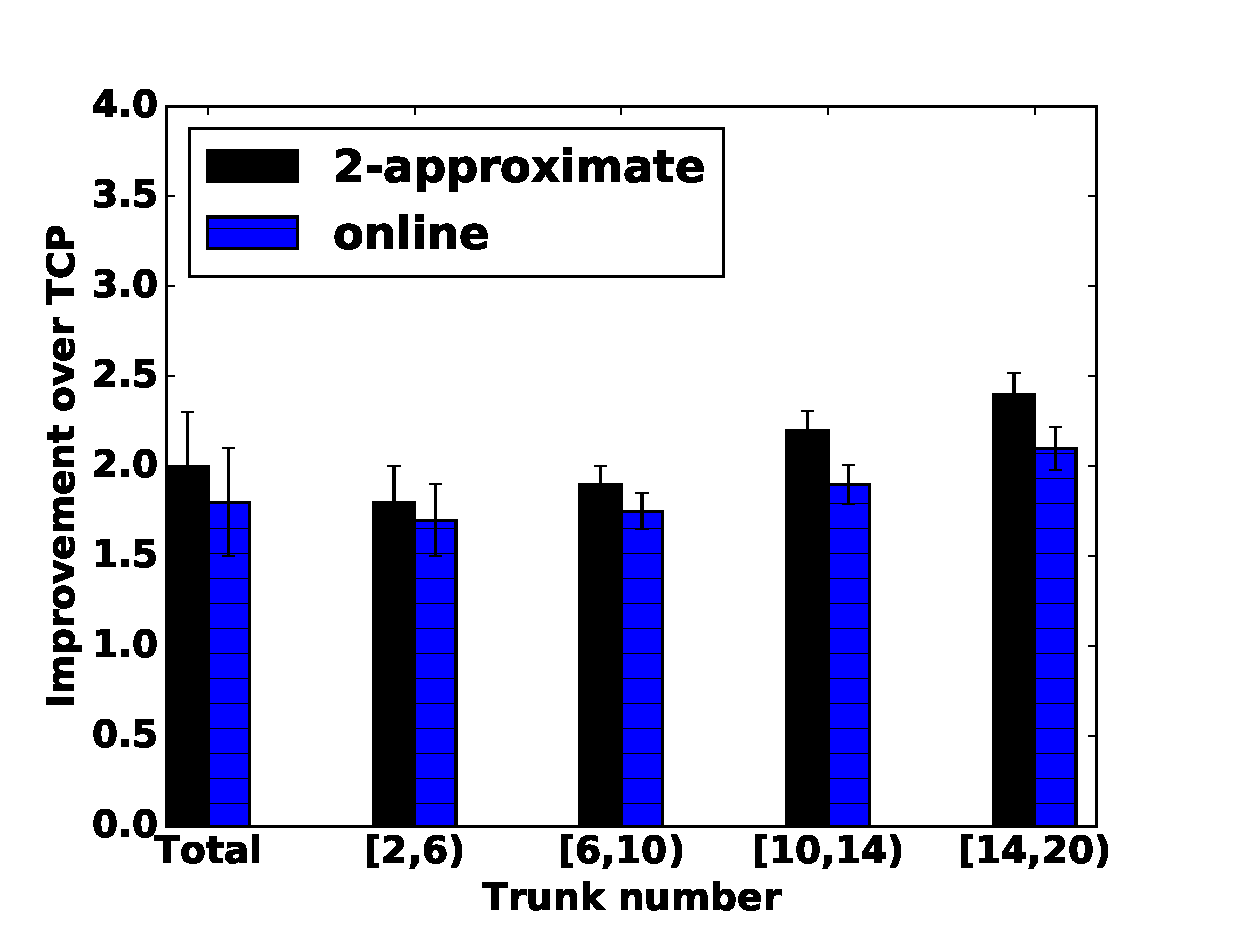
\includegraphics[width=0.5\columnwidth]{figures/DTARGET/picture/evaluation/ex3/on_off_3.eps}}%
  %\hspace{7em}%
  \subcaptionbox{FAT分布(没有使用SLF)\label{DTARGET_Evaluation_Motivation:subfig4}}
      {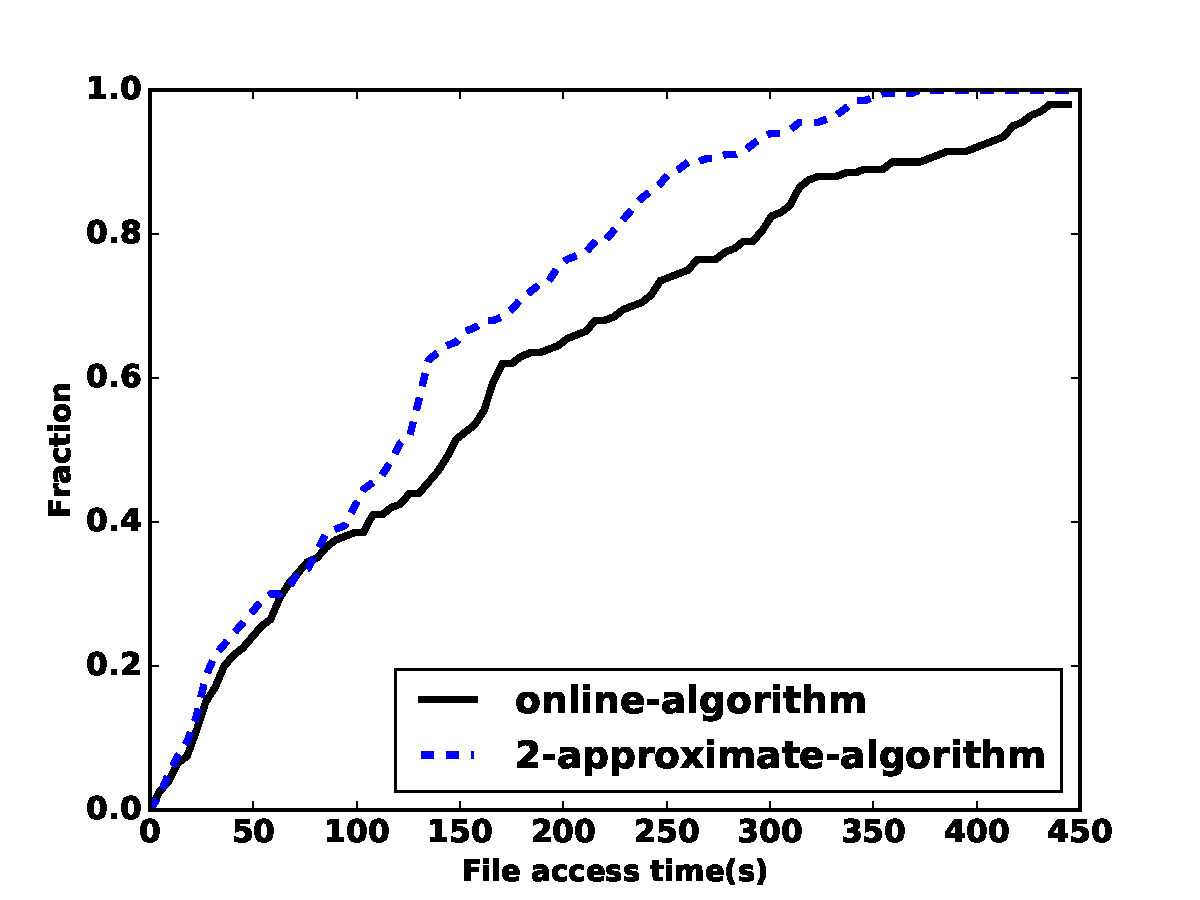
\includegraphics[width=0.5\columnwidth]{figures/DTARGET/picture/evaluation/ex3/online_offline2.pdf}}
  \caption{2-近似的离线算法和在线算法的结果对比,注意TCP被选作基准}
  \label{loss_fig}
\end{figure}


与离线的2-近似算法相比,实时调度的在线算法\ref{online-algorithm}忽略负载的差异性,这可能导致性能损失。
在本节中,研究在线算法和2-近似离线算法之间的性能差距。
使用AT\&T的流量,并设置所有的请求到达时间为t = 0,图\ref{loss_fig}显示实验结果。

从图\ref{loss_fig}(a)中可以看出,当并行块数分别为[2,6],[6,10],[10,14]和[14,20]时,
2-近似方法的相对于TCP提高幅度是2.2$\times$,2.3$\times$,2.43$\times$,2.52$\times$,而在线方法提高幅度是2.1$\times$,1.8$\times$,1.9$\times$,2.2$\times$。
平均起来2-近似方法的相对于TCP提高幅度是2.4$\times$,而在线方法提高幅度是2.1$\times$。
在线方法有大约$15\%$的性能损失。

图\ref{loss_fig}(b)显示了FAT的分布情况,可以看出,两种近似方法中超过$80\%$的FAT小于300s,而在线方法的FAT大于$65\%$。
在线方法有大约$16\%$的性能损失。

图\ref{loss_fig}(c)显示了没有最小负载优先的启发式的两种方法的性能对比,可以看出,
,当并行块数分别为[2,6],[6,10],[10,14]和[14,20]时,
2-近似方法的相对于TCP提高幅度是1.6$\times$,1.7$\times$,1.8$\times$,1.9$\times$,而在线方法提高幅度是1.6$\times$,1.6$\times$,1.7$\times$,1.8$\times$。
平均起来2-近似方法的相对于TCP提高幅度是2.0$\times$,而在线方法提高幅度是1.6$\times$。
在线方法有大约$20\%$的性能损失。

图\ref{loss_fig}(d)显示了FAT的分布,可以看到,
不使用SLF情形下,在线的调度方法大约$80\%$的FAT在350s以内,这比SLF的方法差$28\%$左右。

\section{本章总结}
本章中提出了基于流信息的任务级传输优化方法对任务级的传输进行优化,
并且提出最小化负载有限的启发式方法对纠删码存储系统进行访问优化。 
本章的优化目标是最小化文件平均访问时间(Average File Access Time,简称AFAT)。 
首先,本章提出理想情况下的文件访问时间最小化(Idealized File Access Time Minimization,简称IFATM)问题,
随后,将此问题简化,得到简单理想情况下的文件访问时间最小化(Simple Idealized File Access Time Minimization,简称SIFATM)问题,研究其复杂度,并导出近似优化的非抢先式调度算法,证明其近似度。
随后,本章设计在线调度策略,并且设计并实现了D-Target,一个集中式的调度器,并通过真实数据中心流量来评估D-Target的性能。
